\chapter{Desenvolvimento} \label{cap:desenvolvimento}

Diante da relevância do tema e do raciocínio exposto, foi desenvolvido um método para análise de \index{Vulnerabilidade} vulnerabilidades em redes industriais \index{OPC UA} OPC UA. Este capítulo apresenta os principais aspectos da bancada experimental utilizada, bem como o conjunto de estratégias adotado para sua implementação e desenvolvimento.

\section{Aspectos da Bancada Experimental para Ensaios de Intrusão em Redes OPC UA}

    Nesta seção, descreve-se a estrutura responsável pela aquisição dos dados experimentais gerados para o desenvolvimento deste trabalho. A \autoref{fig:esqBanc} ilustra a composição da bancada experimental, cujos principais componentes são detalhados a seguir.

    \begin{figure}[htbp]
        \caption{\label{fig:esqBanc}Esquema geral da bancada experimental para ensaios de segurança cibernética}
        \begin{center}
            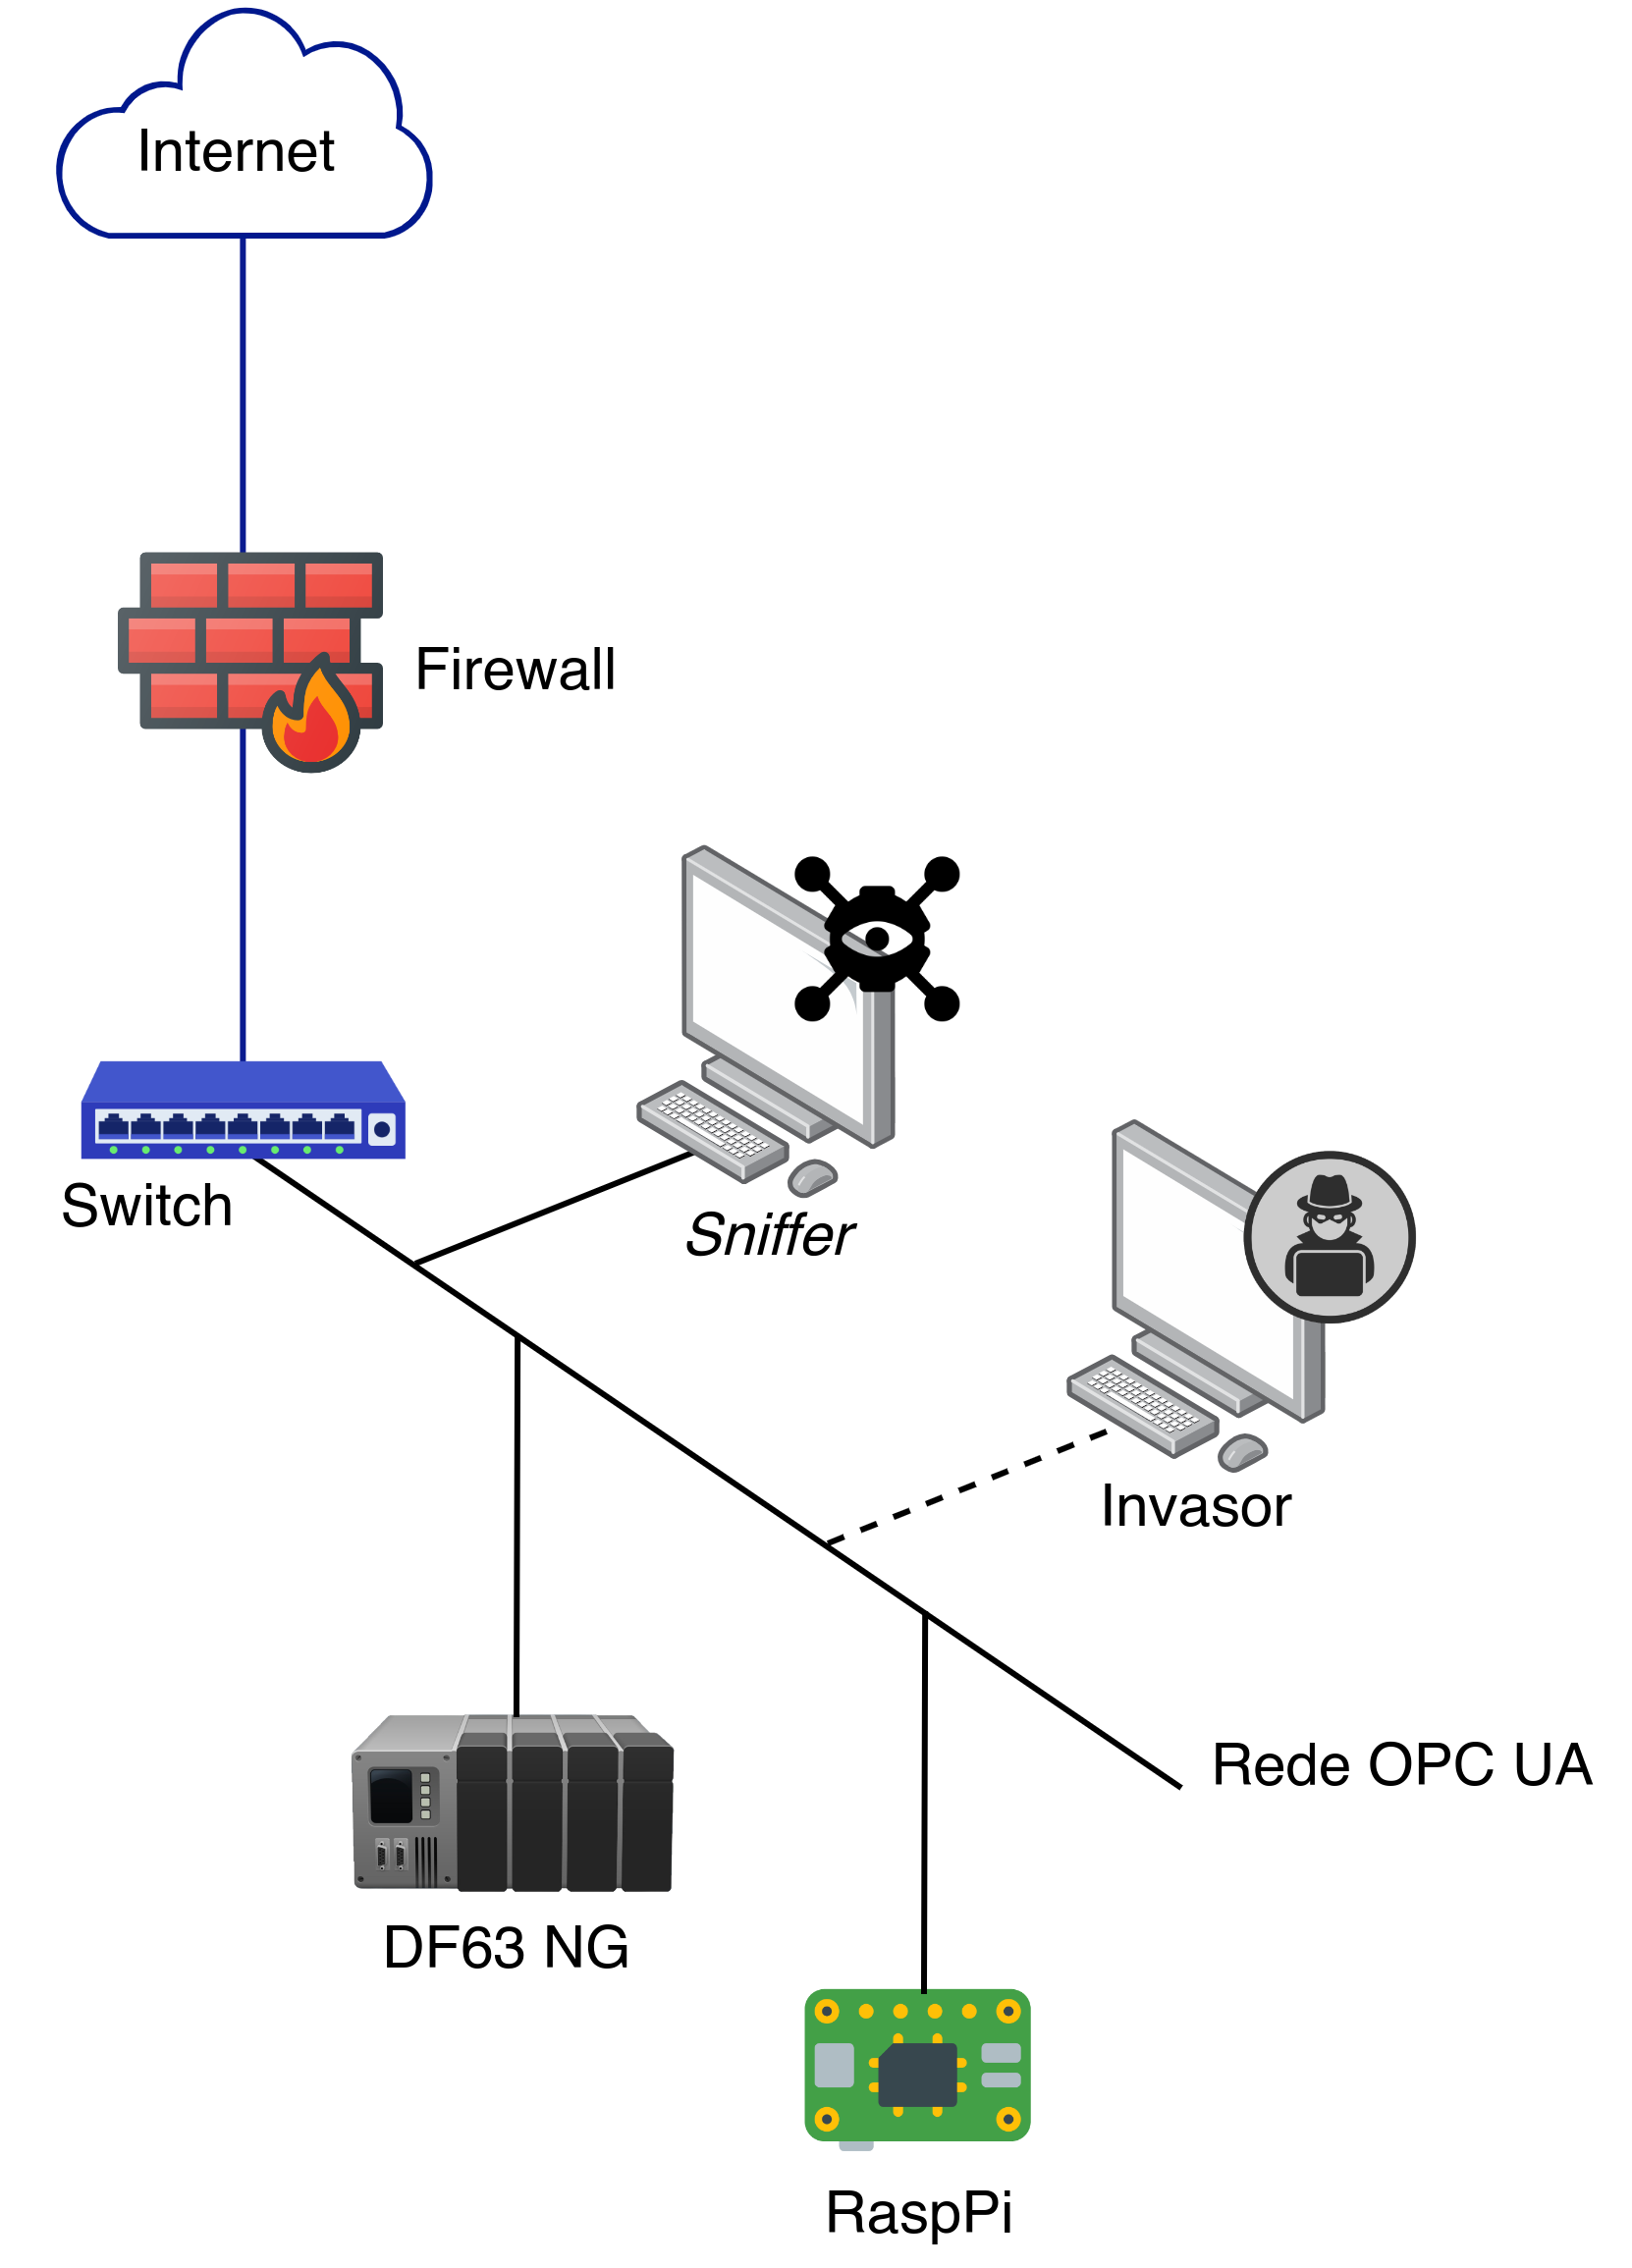
\includegraphics[width=0.6\textwidth]{USPSC-img/bancada.png}
        \end{center}
        \legend{Fonte: elaborada pelo autor.}
    \end{figure}

    \subsection{\textit{Hardware}}

        Para simular ataques cibernéticos, é necessário um conjunto de componentes de \textit{hardware} combinado com ferramentas de \textit{software} específicas. A seguir, são apresentados os equipamentos utilizados:

        \begin{itemize}
            \item \underline{DF63 NG}: controlador multifuncional da nova geração da plataforma DFI302 da Nova Smar S/A, projetado para conectar redes H1 independentes a redes Ethernet HSE, atuando como um `\textit{linking device}'. Desenvolvido para soluções de controle distribuído em redes industriais, suporta comunicação Modbus e oferece recursos avançados, como redundância `\textit{Hot standby}', comunicação OPC UA nativa e configuração por meio da linguagem Ladder, conforme a norma IEC 61131. Além disso, a DF63 NG é altamente versátil, permitindo a instanciação de centenas de blocos funcionais, incluindo blocos flexíveis, e conta com um servidor Web integrado para diagnóstico e parametrização;
            \item \underline{Raspberry Pi 4 Modelo B}: mini-computador de placa única configurado com o sistema operacional Kali Linux, utilizado para hospedar um servidor OPC UA. A Raspberry Pi 4 Modelo B representa um avanço significativo em relação às versões anteriores, incorporando um processador ARM Cortex-A72 quad-core de 64 bits, com clock de 1,5 GHz, suporte a Wi-Fi 802.11ac, Bluetooth 5.0 e maior capacidade de memória. Esses aprimoramentos garantem um ambiente experimental mais robusto e com maior capacidade de processamento para a realização dos testes de intrusão em redes OPC UA;
            \item \underline{\textit{Ethernet Switch}}: dispositivo de rede essencial para centralizar a comunicação entre múltiplos equipamentos. Utiliza a técnica de comutação de pacotes para receber e encaminhar dados entre dispositivos. Neste projeto, emprega-se um \textit{switch} Ethernet da marca TP-Link para estabelecer a conexão entre os clientes OPC UA e o servidor. O servidor OPC UA está conectado ao \textit{switch} por meio de um cabo LAN, assim como o dispositivo que hospeda o cliente OPC UA. Destaca-se que os \textit{switches} da TP-Link incorporam tecnologia Ethernet verde, proporcionando economia de energia, enquanto o controle de fluxo IEEE 802.3x assegura uma transferência de dados confiável;
            \item \underline{Elemento Invasor}: desempenha um papel central na realização dos testes de intrusão deste estudo, simulando ataques cibernéticos. Trata-se de um computador configurável para diferentes cenários de teste, no qual são executadas ferramentas de análise e ataque, como Hping3 e Nmap (veja \autoref{subsec:software}). Ressalta-se que o Elemento Invasor é empregado exclusivamente em um ambiente controlado, garantindo que os testes sejam conduzidos com rigor técnico e respeito às normas de segurança. Além disso, as ações realizadas não configuram qualquer violação das diretrizes estabelecidas pela Lei Geral de Proteção de Dados (LGPD), uma vez que não são aplicadas em redes ou implementações reais.
        \end{itemize}
    
    \subsection{\textit{Software}} \label{subsec:software}

        Um conjunto de ferramentas de \textit{software} é essencial para a realização dos ataques às redes OPC UA. As principais são descritas a seguir:

        \begin{itemize}
            \item \underline{Smar OPC UA Server}: servidor OPC UA proprietário da Nova Smar S/A, amplamente empregado no setor industrial em conjunto com a linha de produtos compatíveis com o padrão O-PAS (do inglês, \textit{Open Process Automation™ Standards}), desenvolvido pelo OPAF (\textit{Open Process Automation™ Forum}). Proporciona um ambiente altamente seguro e eficiente para a comunicação e troca de dados em sistemas de automação industrial. A Nova Smar S/A segue aprimorando seu servidor OPC UA para atender às crescentes exigências do mercado, oferecendo uma solução de conectividade robusta e confiável;
            \item \underline{opcua-asyncio}: implementação de código aberto do OPC UA, desenvolvida em Python com suporte para \textit{asyncio}. Licenciada sob a GNU Lesser General Public License v3.0, permite integração e distribuição com \textit{software} proprietário. Essa biblioteca é compatível com diversos ambientes Python e fornece uma implementação detalhada de clientes e servidores OPC UA. O \textit{opcua-asyncio} suporta o conjunto de protocolos binários OPC UA, além de incluir um SDK para desenvolvimento de clientes e servidores, sendo uma alternativa flexível para desenvolvedores que utilizam Python;
            \item \underline{OPC UA Exploit Framework}: projeto de código aberto desenvolvido e mantido pela Claroty Team82, que fornece um conjunto avançado de ferramentas para pesquisa e exploração de vulnerabilidades em redes OPC UA. Seu principal objetivo é apoiar empresas desenvolvedoras de \textit{software} e fornecedoras de OPC UA na fase de testes e aprimoramento de seus produtos, além de auxiliar pesquisadores na identificação e análise de vulnerabilidades e \textit{bugs} sistêmicos;
            \item \underline{Ettercap}: ferramenta utilizada principalmente para a execução de ataques do tipo MITM (\textit{Man-in-the-Middle}). Dispõe de recursos para captura de tráfego em tempo real, filtragem de conteúdo e análise de \textit{hosts} de destino. No contexto deste trabalho, o Ettercap é empregado na implementação do primeiro cenário de ataque, interceptando a comunicação entre cliente e servidor OPC UA;
            \item \underline{Hping3}: ferramenta de linha de comando para montagem e análise de pacotes TCP/IP. Inicialmente desenvolvida para ataques de negação de serviço (DoS), tornou-se amplamente utilizada em testes de segurança de redes. Oferece suporte a protocolos TCP, UDP e ICMP, além de um modo de rastreamento de rota (\textit{traceroute});
            \item \underline{Wireshark}: \textit{software} de código aberto destinado à captura e análise de pacotes e protocolos de rede. É amplamente empregado na solução de problemas de conectividade, no desenvolvimento e análise de protocolos de comunicação e na investigação de tráfego malicioso. Neste trabalho, é utilizado em conjunto com um computador configurado como \textit{sniffer};
            \item \underline{Nmap}: ferramenta gratuita e de código aberto utilizada para varredura de redes e detecção de portas abertas. Permite a identificação de \textit{hosts} e serviços em uma rede, bem como a verificação de detalhes como o tipo de serviço em execução e o status das portas. Seu funcionamento baseia-se no envio de pacotes ao alvo e posterior análise das respostas.
        \end{itemize}

\section{Ataques Cibernéticos em Redes Industriais OPC UA} \label{sec:attacks}

    Nesta seção, apresenta-se uma análise detalhada dos cenários de ataque implementados neste projeto. A exposição abrange uma descrição passo a passo das metodologias empregadas para orquestrar três formas distintas de ciberataques: interceptação de pacotes (\textit{Packet Sniffing}), ataques do tipo MITM e negação de serviço. Ao elucidar as complexidades desses vetores de ataque, busca-se fornecer uma compreensão aprofundada das ameaças emergentes à cibersegurança em redes OPC UA.

    \subsection{\textit{Packet Sniffing}}

        Após a instalação e operação da rede OPC UA nos dispositivos envolvidos, o invasor inicia o \textit{software} Ettercap, utilizando-o como um \textit{sniffer} para capturar e analisar o tráfego de rede. O modo unificado do Ettercap permite a execução do ataque por meio de uma única interface de rede. Para viabilizar essa interceptação, o invasor deve estar conectado à mesma rede de comunicação OPC UA e a uma porta de um \textit{switch} gerenciável, configurado para replicar o tráfego de dados entre o cliente e o servidor OPC UA. Essa configuração possibilita a captura e a inspeção dos pacotes transmitidos, conforme ilustrado na \autoref{fig:sniffing}.

        \begin{figure}[htbp]
            \caption{\label{fig:sniffing}Esquemático do ataque \textit{Packet Sniffing}}
            \begin{center}
                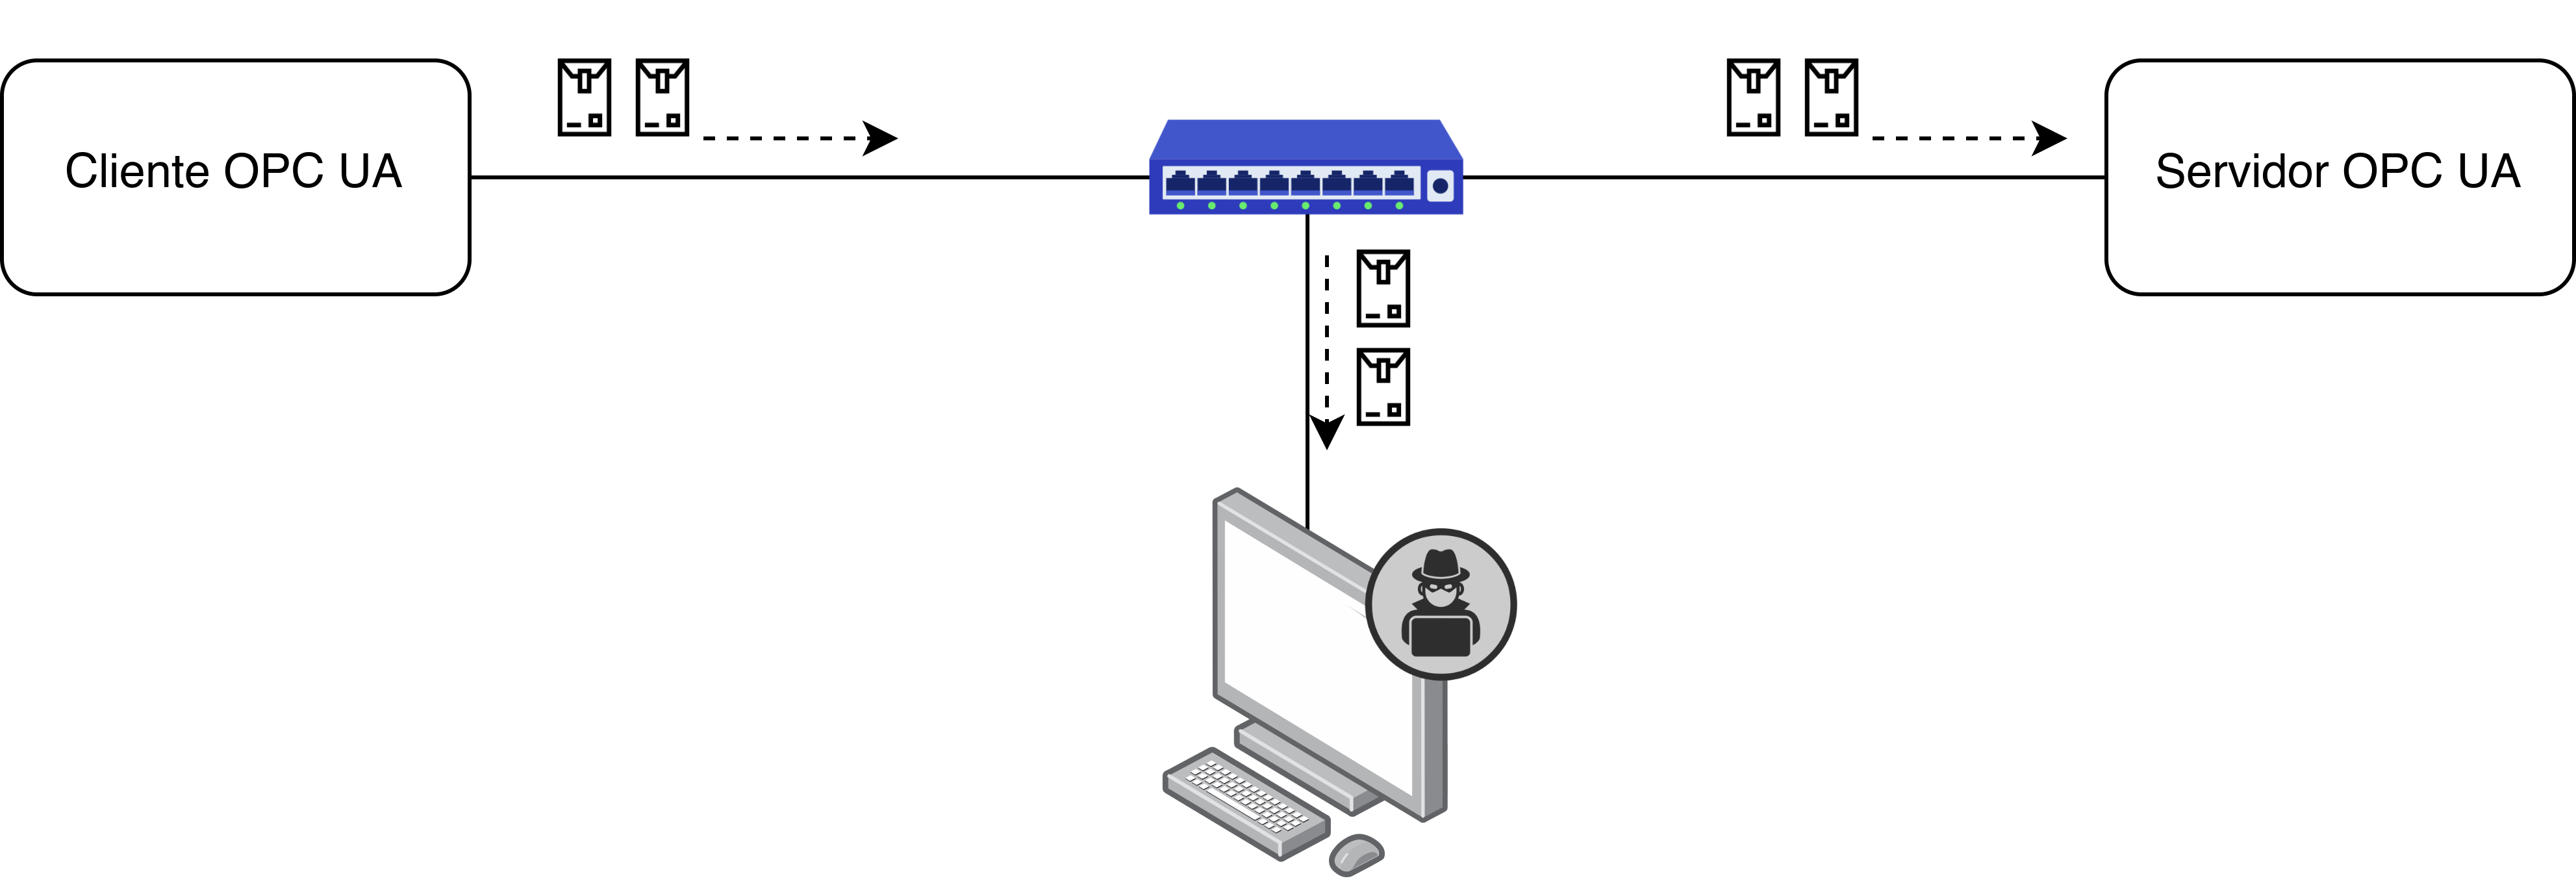
\includegraphics[width=0.9\textwidth]{USPSC-img/sniffing.png}
            \end{center}
            \legend{Fonte: elaborada pelo autor.}
        \end{figure}
        
        Com o início da operação de \textit{sniffing} pelo Ettercap, o Wireshark é empregado para uma análise mais detalhada dos endereços capturados. A \autoref{fig:sniffWire} apresenta a sequência de pacotes registrados pelo \textit{software} quando a interceptação do tráfego de rede ocorre com sucesso. Detalhes adicionais sobre a análise dos dados obtidos nesse processo são apresentados no \autoref{cap:resultados}.

        \begin{figure}[htbp]
            \caption{\label{fig:sniffWire}Resultados de captura do Wireshark durante o \textit{sniffing} de pacotes}
            \begin{center}
                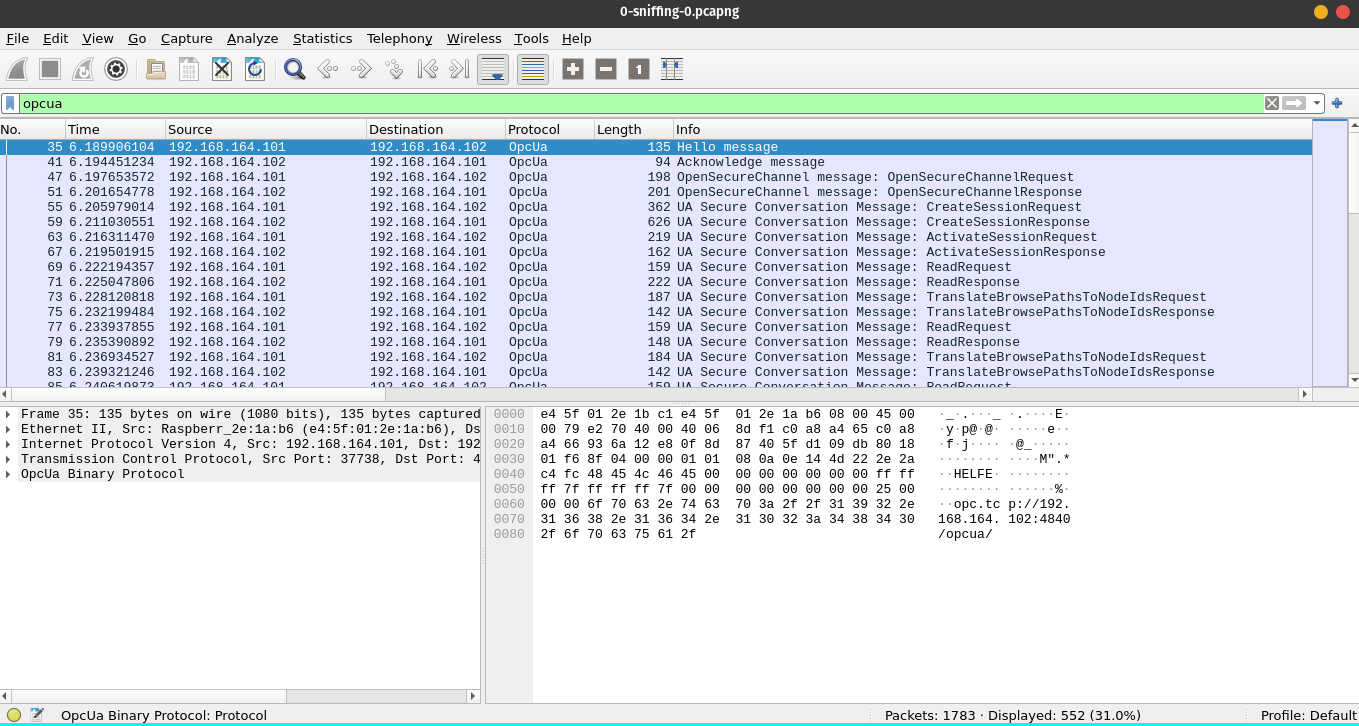
\includegraphics[width=1\textwidth]{USPSC-img/sniffWire.png}
            \end{center}
            \legend{Fonte: elaborada pelo autor.}
        \end{figure}
    
    \subsection{\textit{Man in the Middle (MITM)}}

       No ataque MITM, o invasor é capaz de interceptar informações transmitidas pelo \textbf{SecureChannel} entre o cliente e o servidor OPC UA, conforme ilustrado na \autoref{fig:mitm}.

        \begin{figure}[htbp]
            \caption{\label{fig:mitm}Esquemático do ataque MITM}
            \begin{center}
                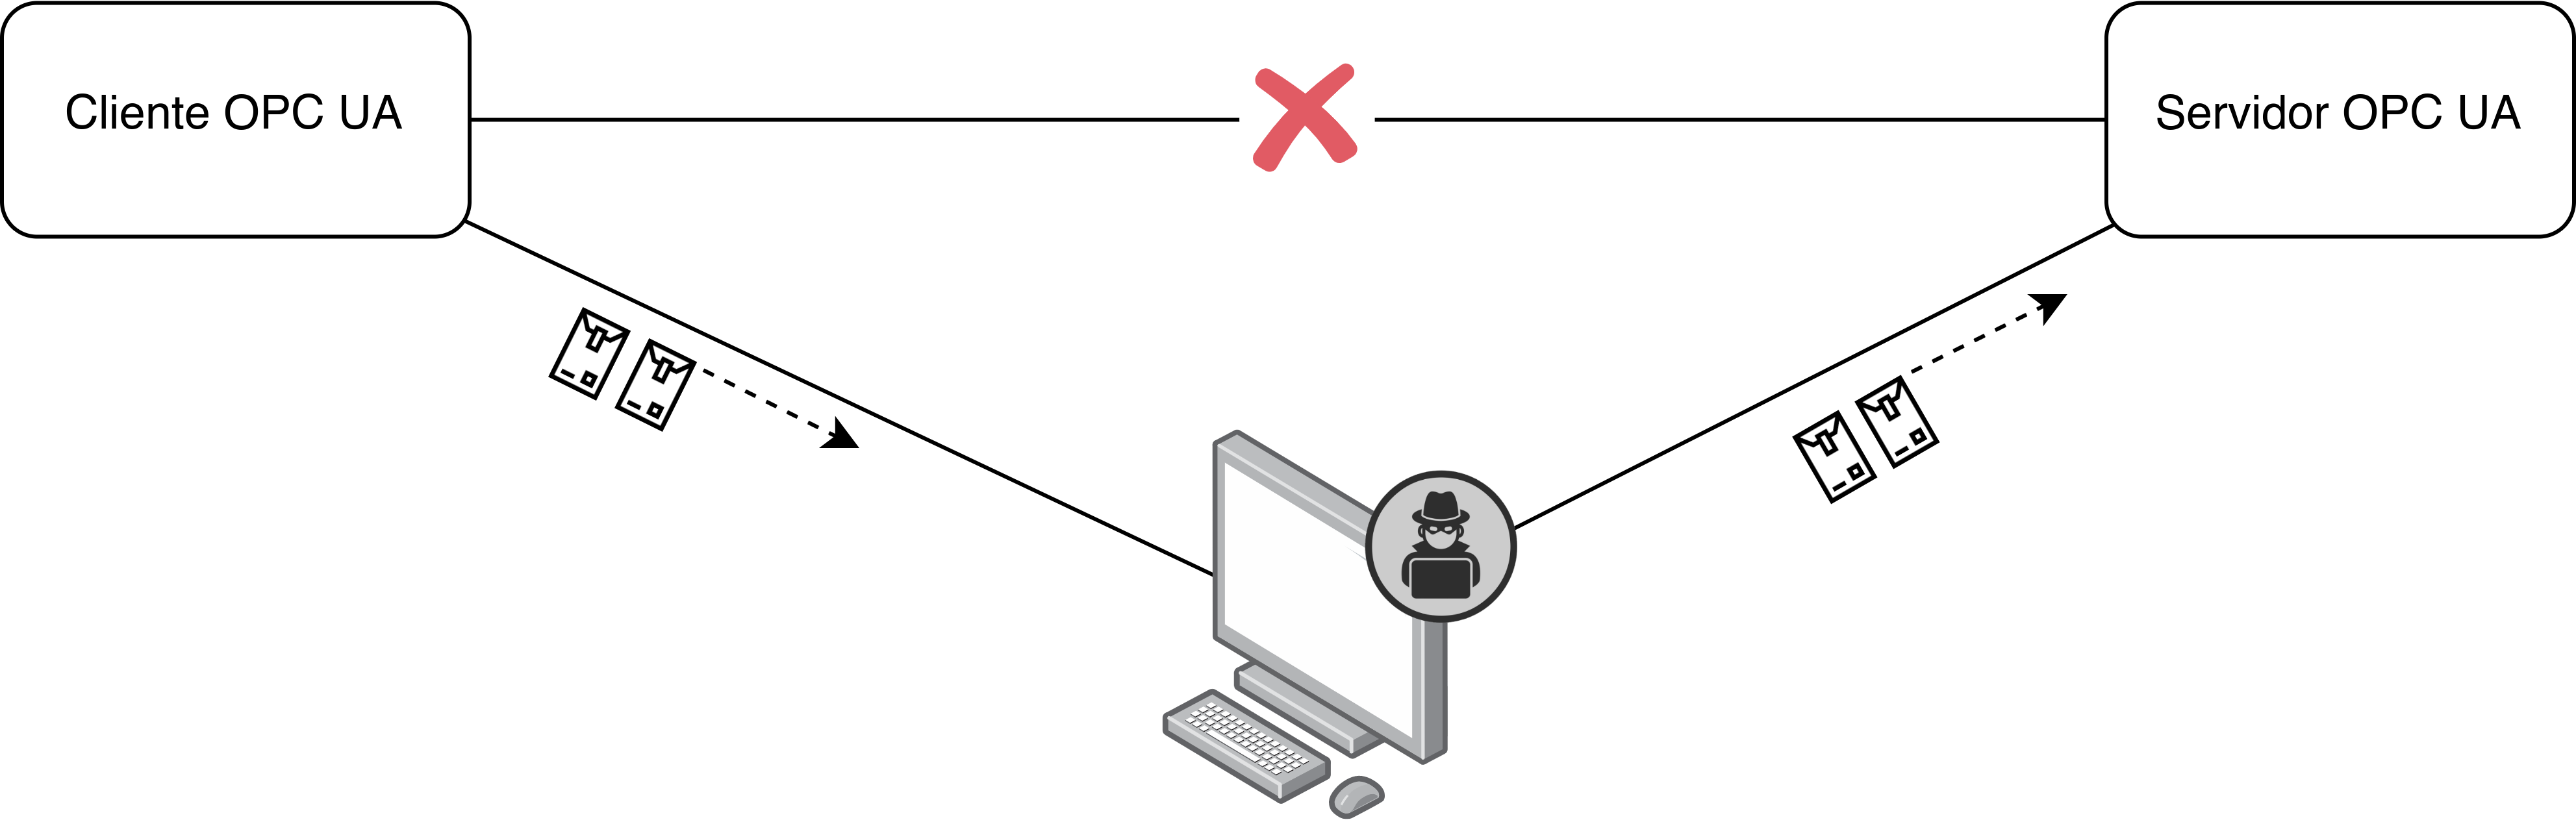
\includegraphics[width=0.9\textwidth]{USPSC-img/mitm.png}
            \end{center}
            \legend{Fonte: elaborada pelo autor.}
        \end{figure}
        
        
        A primeira etapa desse ataque consiste em uma varredura da rede, realizada com a ferramenta Ettercap. Durante esse procedimento, a busca por \textit{hosts} ativos abrange todos os endereços pertencentes à máscara de rede configurada. Por exemplo, caso a máscara seja 255.255.255.0 (/24), um total de 256 endereços será analisado para identificar quais dispositivos estão em funcionamento.

        Após a conclusão da varredura, o invasor seleciona os alvos do ataque MITM e prossegue com a falsificação de endereços ARP (do inglês \textit{ARP Spoofing}), um dos métodos mais utilizados para esse tipo de ataque. O protocolo ARP (do inglês \textit{Address Resolution Protocol}) desempenha um papel essencial na camada de rede do modelo OSI, permitindo a associação de endereços IP a endereços MAC (do inglês \textit{Media Access Control}). No \textit{ARP Spoofing}, o invasor envia respostas ARP maliciosas à rede, anunciando falsamente que seu endereço MAC corresponde aos endereços IP do roteador e da estação de trabalho. Dessa forma, ambos os dispositivos atualizam suas tabelas ARP e passam a redirecionar seu tráfego ao invasor, que, a partir desse ponto, consegue interceptar e manipular os pacotes transmitidos entre eles.

        Além do ataque por falsificação de ARP, também foi realizado um ataque MITM por roubo de portas (do inglês \textit{port stealing}) utilizando a ferramenta Ettercap. Nesse método, o invasor captura o tráfego entre o cliente e o servidor OPC UA ao inundar a rede com pacotes ARP, nos quais o endereço MAC de destino corresponde ao próprio invasor e o endereço MAC de origem pertence à vítima. Como consequência, a porta do \textit{switch} associada ao alvo é ``roubada'', permitindo que os pacotes destinados a ela sejam desviados para o invasor. Em seguida, o invasor interrompe a inundação, envia uma solicitação ARP ao destino real do pacote e, ao receber a resposta, reencaminha o pacote interceptado. Esse processo é repetido continuamente para garantir a captura de dados sem interromper a comunicação entre os dispositivos.

        Enquanto os ataques MITM por falsificação de ARP e roubo de portas são conduzidos pelo Ettercap, a captura dos pacotes é realizada simultaneamente pelo Wireshark. Para facilitar a análise desenvolvida neste estudo, o Wireshark é configurado para filtrar pacotes do protocolo OPC UA, permitindo uma inspeção detalhada das comunicações estabelecidas na rede.

    \subsection{\textit{Denial of Service (DoS)}}

        Esse tipo de ataque permite que o Elemento Invasor insira clientes não confiáveis na rede OPC UA, além de possibilitar a inundação da rede e do servidor por meio do envio contínuo de mensagens específicas. A \autoref{fig:dos} ilustra o funcionamento básico de um ataque DoS, no qual as solicitações oriundas de um cliente OPC UA não confiável são interpretadas pelo servidor, mas rejeitadas devido à falsificação de endereço.

        \begin{figure}[htbp]
            \caption{\label{fig:dos}Esquemático do ataque DoS}
            \begin{center}
                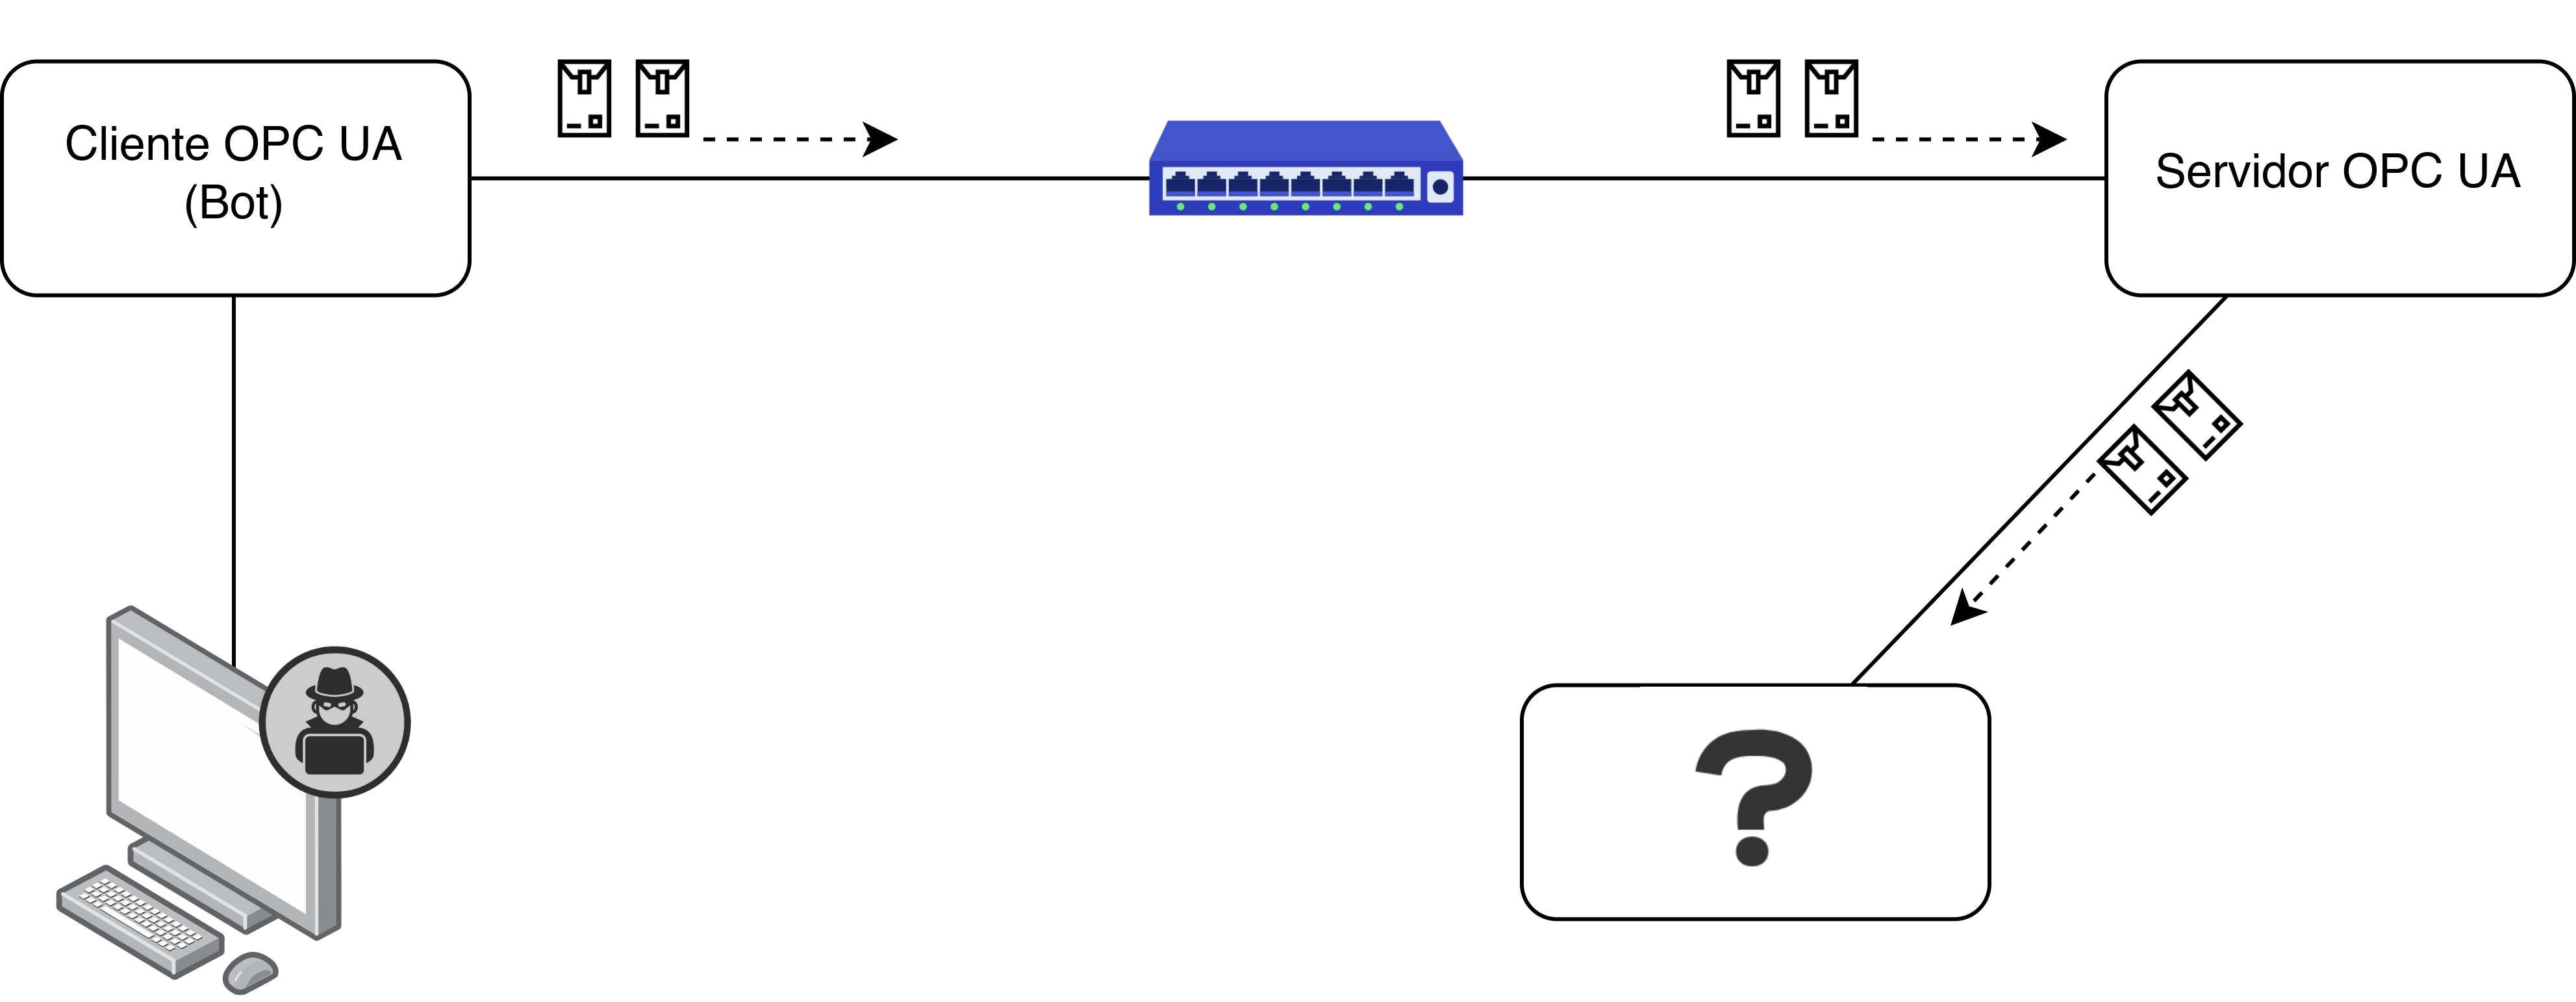
\includegraphics[width=0.9\textwidth]{USPSC-img/dos.png}
            \end{center}
            \legend{Fonte: elaborada pelo autor.}
        \end{figure}
        
        Diversos cenários podem ser explorados para a execução de um ataque de negação de serviço. Além do impacto causado pela inundação da rede, destaca-se a sobrecarga no processamento do servidor, especialmente em ataques intensivos, nos quais ele precisa validar certificações para responder às solicitações. Segundo \citeonline{neu2019}, os principais cenários incluem:

        \begin{enumerate}
            \item \underline{SYN \textit{Flooding}}: o cliente sobrecarrega o servidor enviando continuamente mensagens SYN, às quais o servidor responde com mensagens ACK. Embora esse ataque possa aumentar significativamente o tráfego na rede, seu impacto no consumo de recursos do servidor é relativamente limitado;
            \item \underline{ACK ou ERR \textit{Flooding}}: nesse cenário, o cliente inunda o servidor com mensagens ACK e/ou ERR, forçando-o a responder com mensagens ERR. Assim como no caso anterior, ocorre uma sobrecarga na rede, mas o impacto nos recursos computacionais do servidor permanece moderado;
            \item \underline{Inundação com Mensagens Incorretas}: o Elemento Invasor envia continuamente mensagens inválidas, obrigando o servidor a responder com mensagens ERR. Esse ataque também resulta em um aumento do tráfego na rede, mas seu efeito sobre o processamento do servidor é relativamente reduzido;
            \item \underline{CLO \textit{Flooding}}: mensagens repetitivas de solicitação de fechamento de canal (CLO) são enviadas ao servidor, que responde com mensagens ERR, contribuindo para a sobrecarga da rede;
            \item \underline{Inundação com \textbf{FindServers} ou \textbf{GetEndpoints}}: o cliente estabelece um canal no modo de segurança ``None'' e, em seguida, envia continuamente mensagens \textbf{FindServers()} ou \textbf{GetEndpoints()} para o servidor, que responde utilizando o protocolo OPC UA MSG. Esse ataque impacta o tráfego na rede, mas não causa sobrecarga significativa nos recursos do servidor;
            \item \underline{Inundação com Solicitações SYN e OPN}: um cliente não confiável executa um ataque de negação de serviço enviando continuamente solicitações SYN e OPN ao servidor, que responde com mensagens ACK e ERR. Nesse caso, o servidor consome recursos consideráveis ao validar certificados, processar solicitações e criptografar mensagens. O impacto desse ataque é ainda maior quando a Autoridade de Certificação está localizada em um sistema separado, pois o tempo de validação do certificado aumenta significativamente, intensificando a carga sobre o servidor.
        \end{enumerate}

        Para realizar a inundação da rede e viabilizar o ataque DoS, utilizam-se duas ferramentas: OPC UA Exploit Framework e Hping3. Além disso, o Nmap é empregado para mapear a rede, identificando portas abertas e endereços IP disponíveis.

        Uma vez que o Elemento Invasor obtém acesso a um dos componentes da rede-alvo, o Nmap é utilizado para mapeamento da infraestrutura. O comando a seguir executa uma varredura SYN em um intervalo de endereços IP. Esse procedimento é relativamente discreto e difícil de detectar, pois não completa a conexão TCP. Também conhecido como escaneamento de portas entreabertas (\textit{half-open scanning}), esse método consiste no envio de um pacote SYN simulando a abertura de uma conexão real, aguardando uma resposta. Caso o servidor retorne um SYN/ACK, significa que a porta está ativa (aberta); se responder com um RST (\textit{reset}), a porta é considerada inativa. Caso nenhuma resposta seja recebida após múltiplas tentativas, a porta é classificada como filtrada. Da mesma forma, se um erro ICMP indicando inacessibilidade for retornado, a porta também será considerada filtrada.

        \begin{minted}[
            breaklines,
            %linenos,
            mathescape,
            encoding=utf8,
            framesep=2mm,
            baselinestretch=1.2,
            bgcolor=codeback,
            fontsize=\footnotesize
        ]{console}
nmap -sS 192.168.164.*
        \end{minted}

        A execução bem-sucedida desse mapeamento resulta em uma lista de endereços IP disponíveis e respectivas portas abertas, que servirão como base para as etapas subsequentes. O Hping3 é empregado para realizar o ataque de SYN \textit{Flooding} (1) na rede. Para isso, o Elemento Invasor deve implementar o seguinte \textit{script} de configuração, personalizando-o de acordo com o cenário específico.


        \begin{minted}[
            breaklines,
            %linenos,
            mathescape,
            encoding=utf8,
            framesep=2mm,
            baselinestretch=1.2,
            bgcolor=codeback,
            fontsize=\footnotesize
        ]{bash}
# CONFIGURAÇÃO
set TARGET "192.168.164.101"  # O alvo do ataque
set FAKEIP "192.168.164.201"  # Endereço falso
set BROADCAST "192.168.164.254"  # Endereço de broadcast da rede

set PORTS {{4840}{4192}}  # Utilizar as portas abertas encontradas no Nmap
set PORTUDP 123  # Utilizar uma porta UDP ativa

set commandRunTime 60

# EXECUÇÃO
foreach port $PORTS {
    lappend commands "hping3 -S -a $FAKEIP -p $port --flood -V $TARGET"
}
        \end{minted}

        Com o \textit{script} devidamente configurado, o Hping3 está preparado para iniciar o ataque direcionado ao endereço e às portas especificadas, com uma frequência predefinida de sessenta segundos. A interpretação dos parâmetros utilizados na execução é a seguinte: o argumento \textbf{-S} define o tipo de ataque; \textbf{-p} especifica a porta de destino; \textbf{-V} indica o endereço IP do alvo; e \textbf{-a} determina o endereço IP falsificado utilizado no ataque, estratégia que pode ser eficaz para contornar \textit{firewalls}.

        Por fim, ataques mais sofisticados são executados com o auxílio da ferramenta OPC UA Exploit Framework. Os ataques de negação de serviço disponibilizados por esse \textit{framework}, selecionados para execução no ambiente de simulação industrial proposto, são apresentados a seguir, juntamente com suas respectivas categorias, conforme descrito por \citeonline{neu2019}:

        \begin{itemize}
            \item[N/A] \underline{Loop infinito na cadeia de certificados}: ocorre quando um servidor implementa a verificação da cadeia de certificados sem mecanismos de proteção contra loops infinitos. Esse cenário pode surgir, por exemplo, quando o certificado A é assinado pelo certificado B, que, por sua vez, é assinado pelo certificado A, criando uma dependência circular que resulta em um loop infinito durante o processo de verificação da cadeia de certificados;
            % \item[(3)] \underline{Inundação por \textit{Chunk}}: envolve o envio de uma quantidade abundante de fragmentos de dados ao servidor sem o envio do fragmento final correspondente. O OPC UA permite a divisão dos dados em fragmentos, comumente chamados como \textit{MessageChunks} ou \textit{Chunks}, que são enviados à medida que são codificados, a fim de facilitar a transmissão e o processamento. Caso ocorra um erro na criação de um destes fragmentos, um \textit{Chunk} final deve ser enviado ao destinatário para notificar o erro, que por sua vez, é marcado com um sinalizador `A' (abortar) para indicar o erro. O receptor deve verificar a segurança do \textit{MessageChunk} abortado antes de processá-lo e, caso esteja tudo certo, ignorar a mensagem, mas sem encerrar o \textbf{SecureChannel};
            \item[(3)] \underline{Desreferenciação de ponteiro nulo}: envolve a invocação de múltiplos métodos OPC UA, seguida pelo encerramento abrupto da sessão antes da conclusão desses métodos. Essa ação força a aplicação servidora a referenciar um objeto nulo ou um ponteiro inválido, levando a um erro de execução;
            \item[(6)] \underline{Abertura de múltiplos canais seguros}: consiste na tentativa de sobrecarregar o servidor enviando um grande número de solicitações \textbf{OpenSecureChannels};
            % \item[(3)] \underline{Mensagem aninhada complexa}: aplicação de uma variante especialmente manipulada e complexa, projetada para explorar vulnerabilidades em um servidor OPC UA. Quando esta variante é processada pelo servidor, ela pode causar um estouro na pilha de chamadas (\textit{call stack overflow}), levando a uma falha no servidor;
            \item[(5)] \underline{Tradução do caminho de navegação}: envolve o envio de requisições para tradução de \textit{browse paths} complexos, explorando a ausência de mecanismos adequados de limitação na resolução desses caminhos. Esse ataque pode resultar em um \textit{call stack overflow}, comprometendo a estabilidade do servidor.
            % \item[Não aplicável] \underline{Falha de espera no \textit{Thread Pool}}: caracteriza uma paralisação (\textit{deadlock}) no sistema de \textit{Thread Pool} -- mecanismo de gerenciamento de \textit{threads} utilizado para processar solicitações de clientes e tarefas no servidor OPC UA -- devido à inanição simultânea de tarefas concorrentes. Em termos mais simples, quando vários processos ou \textit{threads} estão competindo por recursos do \textit{Thread Pools} de um servidor e, devido a problemas de sincronização ou gerenciamento inadequado de \textit{threads}, ficam em um estado de espera prolongado, impedindo efetivamente o servidor de processar solicitações legítimas;
            % \item[(6)] \underline{Persistência ilimitada de subscrições}: inúmeras solicitações de monitoramento ao servidor são enviados por um invasor, todas configuradas para não excluir os itens após o monitoramento. Esta persistência resulta em uma alocação descontrolada de recursos de memória pelo servidor, levando eventualmente a uma negação de serviço devido ao esgotamento de recursos.
            % \item[(3)] \underline{Desreferenciação de ponteiro nulo}: envolve a chamada de vários métodos OPC UA e encerramento da sessão antes da conclusão destes. Isso resulta em uma situação em que a aplicação servidora é forçada a referenciar um objeto nulo ou um ponteiro invalido, levando a um erro de execução;
            % \item[(3)] \underline{Alteração de corrida e navegação no espaçamento de endereço}: o Elemento Invasor realiza a adição de \textit{Nodes} no \textit{Address Space} no servidor e, simultaneamente, remove-os em um ciclo contínuo, enquanto percorre todo o espaçamento de endereço. Esta manobra cria uma situação de competição na qual o servidor está sendo constantemente modificado e examinado ao mesmo tempo, podendo, assim, esgotar os recursos de processamento e resultar em problemas de consistência no \textit{Address Space};
            % \item[(6)] \underline{Atualização de condição ilimitada}: refere-se ao envio repetido e quantidade abundante de chamadas do método \textbf{ConditionRefresh}, o que leva a alocações de memória não controladas e, eventualmente, pode resultar em uma falha no sistema. O método ConditionRefresh é usado para atualizar as condições e estados das variáveis monitoradas em um servidor OPC UA.
        \end{itemize}

        Com base nessas vulnerabilidades, os ataques mencionados podem ser executados por meio da seguinte linha de comando, substituindo SERVER\_TYPE pelo tipo de servidor utilizado (\textit{e.g.}, softing, unified, prosys, kepware, triangle, dotnetstd, open62541, ignition, rust, node-opcua, opcua-python, milo, s2opc), IP\_ADDR pelo endereço IP do alvo, PORT pela porta aberta para comunicação UA, ENDPOINT\_ADDRESS pelo \textit{endpoint} do servidor, FUNC\_TYPE pelo tipo de ataque escolhido (consultar a documentação oficial do \textit{framework} para verificar os nomes das funções disponíveis \cite{claroty2023}) e DIR, parâmetro necessário para algumas funções:

        \begin{minted}[
            breaklines,
            %linenos,
            mathescape,
            encoding=utf8,
            framesep=2mm,
            baselinestretch=1.2,
            bgcolor=codeback,
            fontsize=\footnotesize
        ]{console}
python main.py [SERVER_TYPE] [IP_ADDR] [PORT] [ENDPOINT_ADDRESS] [FUNC_TYPE] [DIR*]
        \end{minted}

\section{Metodologia}

    O fluxograma apresentado na \autoref{fig:flux} ilustra a sequência e a estrutura das atividades, detalhando os passos que compõem a metodologia, os quais serão explanados nas subseções subsequentes.
    
    \begin{figure}[htbp!]
        \caption{\label{fig:flux}Fluxograma da metodologia proposta}
        \begin{center}
            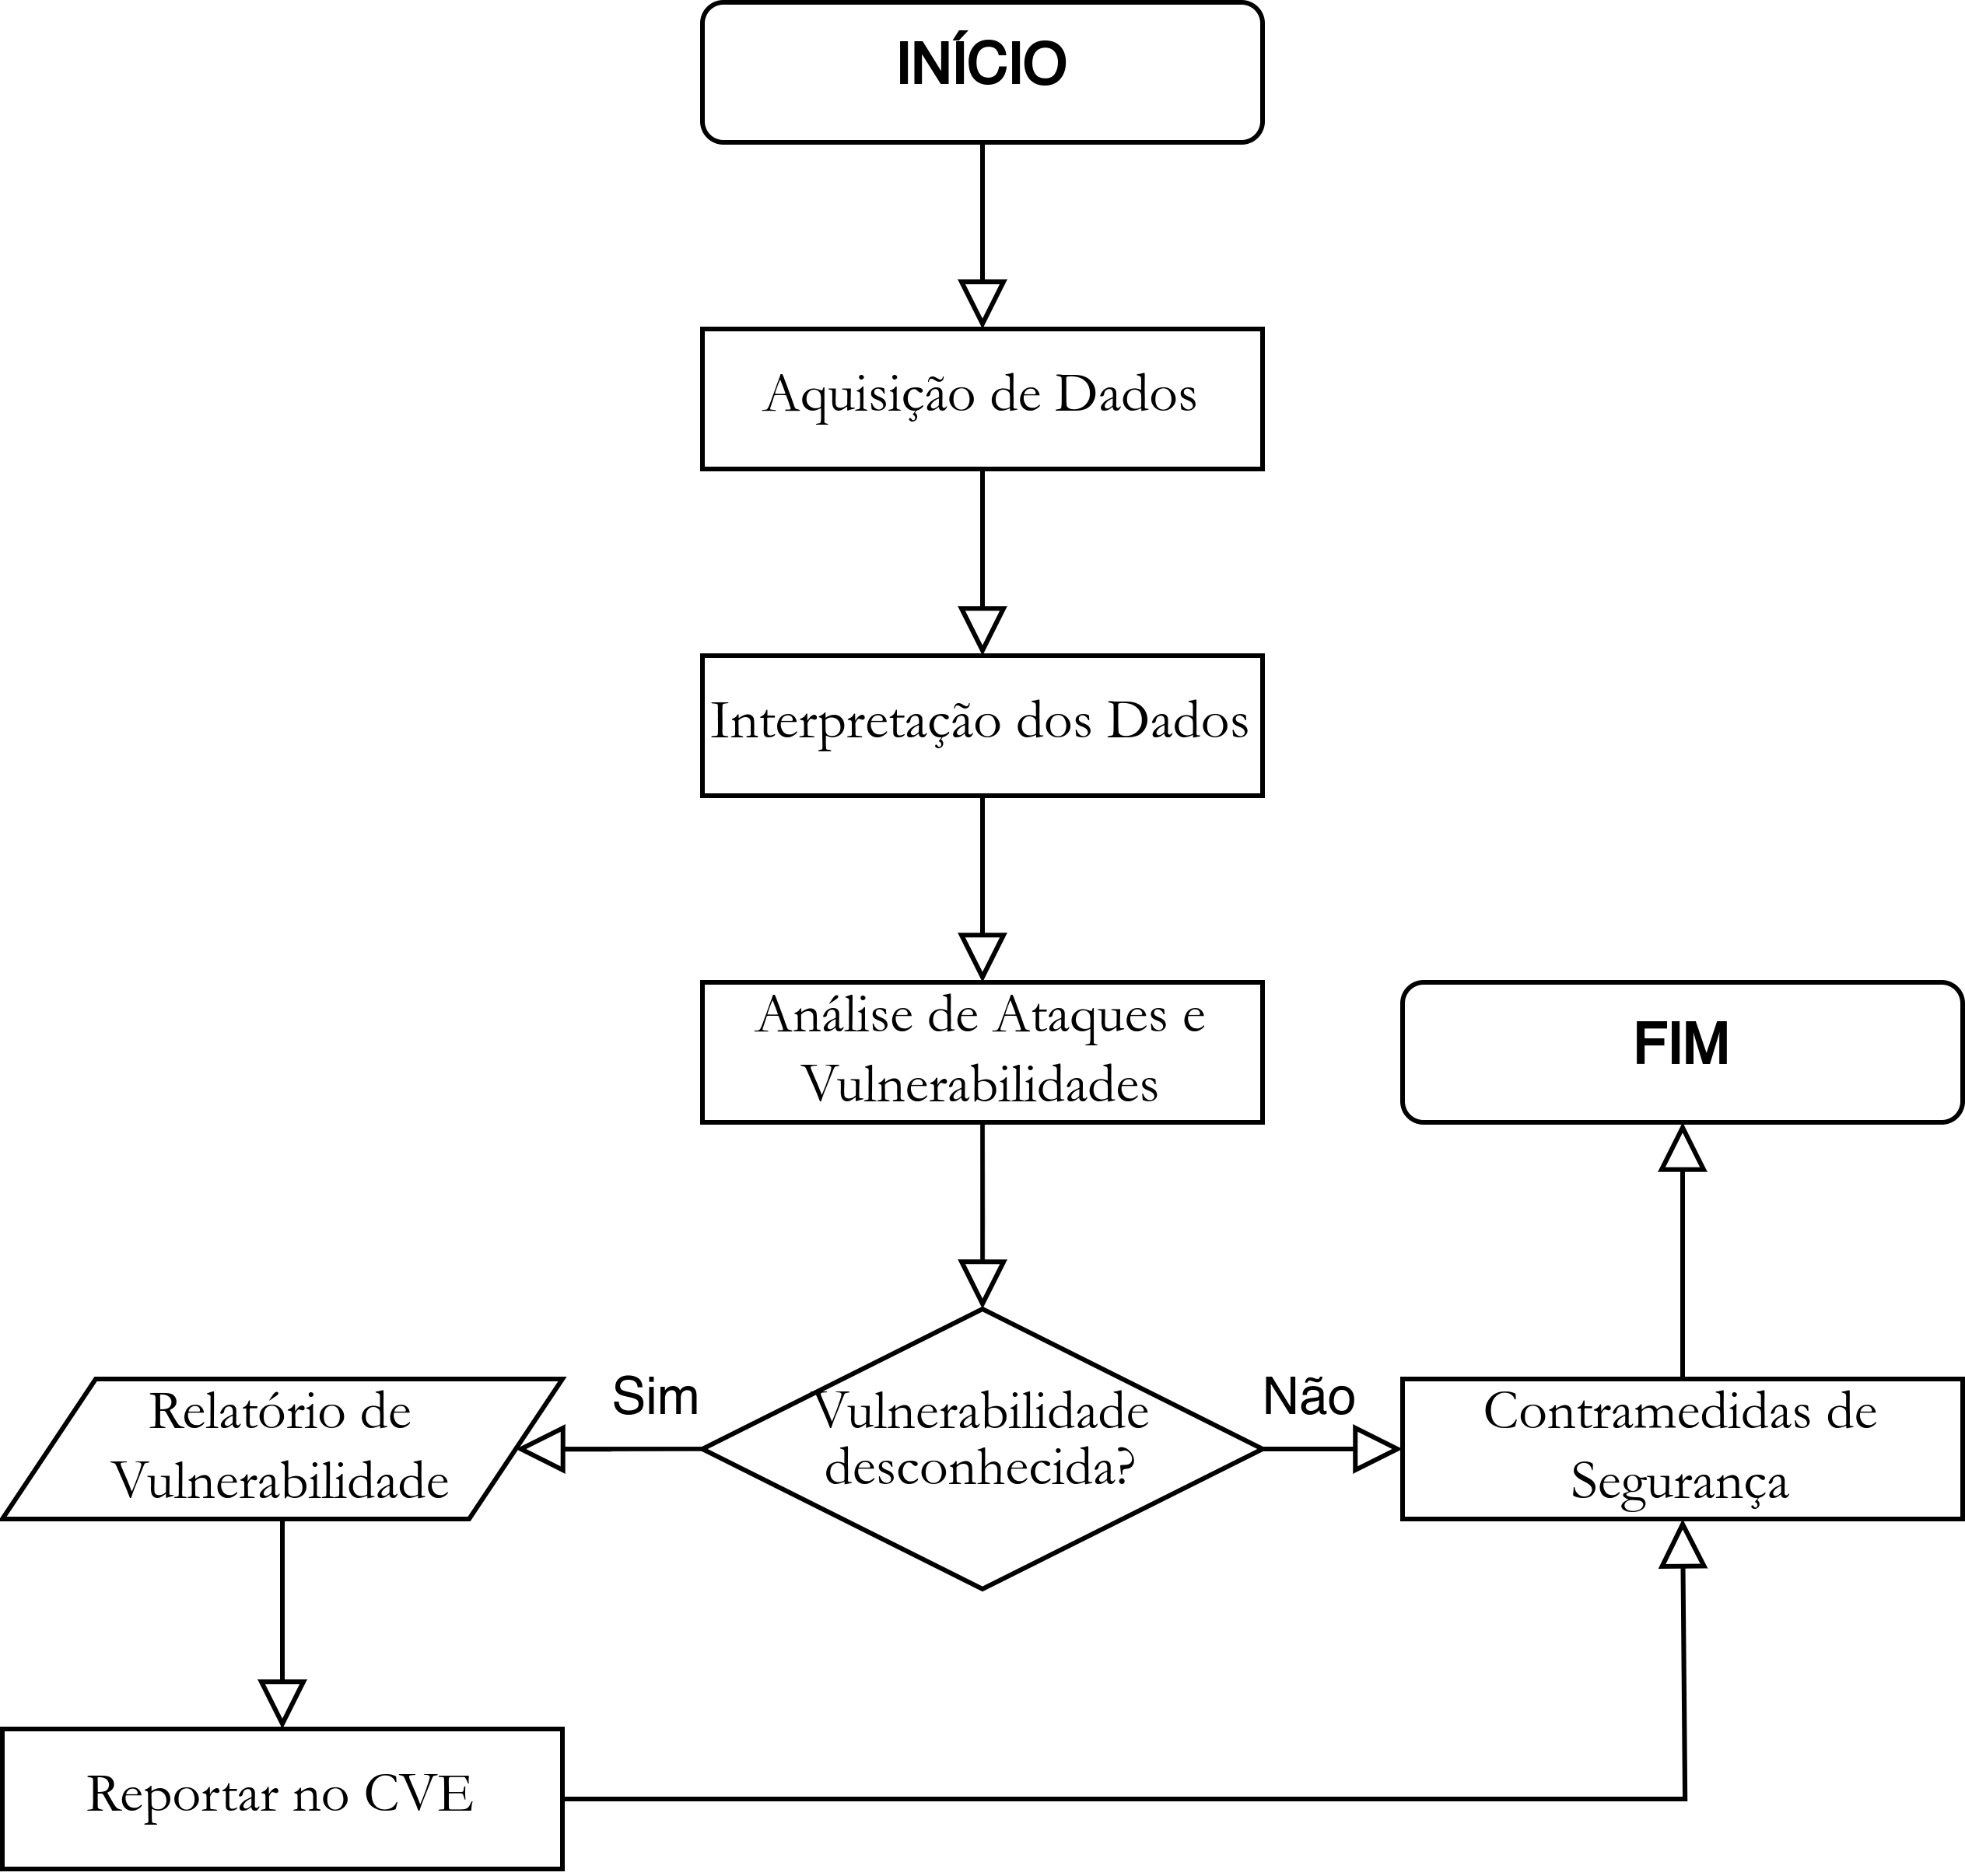
\includegraphics[width=0.7\textwidth]{USPSC-img/fluxograma.png}
        \end{center}
        \legend{Fonte: elaborada pelo autor.}
    \end{figure}

    Para a realização adequada do experimento proposto neste estudo, a infraestrutura de rede do protocolo OPC UA foi configurada conforme os seguintes parâmetros: o Raspberry Pi atuando como servidor e a DF63 NG desempenhando o papel de cliente. Além disso, um elemento de rede denominado \textit{Sniffer} (conforme ilustrado na \autoref{fig:banc}) foi adicionado à configuração para monitorar e registrar a comunicação na rede. Com o objetivo de fornecer uma visão clara dos componentes envolvidos e facilitar a análise dos dados coletados durante o experimento, os endereços IP e MAC de cada elemento do sistema estão resumidos na \autoref{tab:ender}. É importante mencionar que o servidor OPC UA foi configurado para utilizar a porta padrão 4840, e os \textit{endpoints} correspondentes seguem o padrão abaixo. Essa estrutura de configuração foi essencial para a condução eficaz do experimento e a subsequente análise dos resultados.

    Para a correta realização do experimento proposto neste estudo, a infraestrutura de rede do protocolo OPC UA foi configurada conforme os seguintes parâmetros: um Raspberry Pi operando como servidor e a DF63 NG desempenhando a função de cliente. Adicionalmente, um elemento de rede denominado \textit{Sniffer} (conforme ilustrado na \autoref{fig:banc}) foi incorporado à configuração com a finalidade de monitorar e registrar a comunicação na rede. 

    Com o objetivo de proporcionar uma visão clara dos componentes envolvidos e viabilizar a análise dos dados coletados durante o experimento, os endereços IP e MAC de cada elemento do sistema estão sintetizados na \autoref{tab:ender}. Cabe destacar que o servidor OPC UA foi configurado para operar na porta padrão $4840$, e os \textit{endpoints} correspondentes seguem o seguinte formato:

    \begin{minted}[
        breaklines,
        %linenos,
        mathescape,
        encoding=utf8,
        framesep=2mm,
        baselinestretch=1.2,
        bgcolor=codeback,
        fontsize=\footnotesize
    ]{console}
<esquema>://<endereço>:<porta>/<DiscoveryEndpoint>
    \end{minted}

    Onde `<esquema>' pode assumir os valores ``opc.tcp'' ou ``opc.https'', `<endereço>' corresponde ao endereço IP do servidor, `<porta>' refere-se à porta de comunicação OPC UA, e `<DiscoveryEndpoint>' representa o ponto de descoberta do servidor OPC UA.

    \begin{table}[htbp!]
        \centering
        \caption{Endereços IP e MAC dos equipamentos da rede OPC UA}%
        \label{tab:ender}
        \begin{tabular}{ccc}
            \toprule
            \thead{Equipamento} & \thead{IP} & \thead{MAC} \\
            \toprule
            DF63 NG  & 192.168.164.101 & 00:30:5C:24:13:66 \\
            \midrule
            RaspPi   & 192.168.164.102 & E4:5F:01:2E:1A:B6 \\
            % \midrule
            % RaspPi 2 & 192.168.164.102 & E4:5F:01:2E:1B:C1 \\
            \midrule
            Sniffer  & 192.168.164.201 & C8:3A:35:49:FD:58 \\
            \midrule
            Invasor  & 192.168.164.115 & 00:be:43:34:b8:54/00:09:5B:a0:5F:F0 \\
            \bottomrule
        \end{tabular}
        \fonte{elaborada pelo autor.}%
    \end{table}

    Essa configuração foi essencial para a condução eficaz do experimento e para a análise dos resultados no \autoref{cap:resultados}.

    \subsection{Aquisição de Dados} \label{sec:aquisicao}

        A fase de aquisição de dados consiste na captura do tráfego de pacotes transmitidos pela rede OPC UA durante a comunicação entre a aplicação servidora e o cliente, enquanto os ataques são executados. Esse processo é realizado por meio do software Wireshark, que possibilita a obtenção de informações essenciais sobre a comunicação, incluindo detalhes como o tipo de protocolo utilizado, a origem e o destino dos dados. As informações capturadas são armazenadas em ordem cronológica e podem ser salvas em arquivos no formato `.pcapng'. O Wireshark foi configurado para encerrar a captura após sessenta segundos de coleta.

        Os alvos dos ataques são os servidores OPC UA e, em cada cenário, o elemento \textit{Sniffer} é responsável por capturar o tráfego gerado pelos ataques. Para organizar os pacotes capturados, adotou-se a seguinte nomenclatura para os arquivos: `[Modo de Segurança]-[Tipo do Ataque]-[Número da Captura].pcapng'. O modo de segurança pode assumir os valores 0 (None), 1 (Sign) e 2 (Sign\&Encrypt). Os tipos de ataques correspondem àqueles descritos na \autoref{sec:attacks} (``sniffing'', ``mitm'' e ``dos-[função]''), e o número da captura é representado por um dígito de 0 a 9. Por exemplo, para registrar a terceira captura obtida durante um ataque de negação de serviço provocado pela desreferenciação de ponteiro nulo, com a rede configurada no modo de segurança ``Sign'', o arquivo seria nomeado como `1-dos\_function\_call\_null\_deref.pcapng'. A \autoref{tab:attacks} apresenta os cenários analisados e os arquivos de captura gerados durante os experimentos para cada tipo de ataque.

        \begin{table}[htbp]
            \centering
            \caption{Arquivos de captura gerados para cada cenário durante a fase de aquisição de dados}%
            \label{tab:attacks}
            \begin{tabular}{B{1.5cm}B{3cm}B{5.5cm}B{3.5cm}}
            \toprule
                Cenário & Modo de Segurança & Arquivo (.pcapng) & Descrição do Ataque \\
            \end{tabular}
            \begin{tabular}{M{1.5cm}N{3cm}N{5.5cm}N{3.5cm}}
                \toprule
                C1 & None & \code{0-dos\_certificate\_inf\_chain\_loop} & \multirow{3}{*}{\parbox{3.5cm}{DoS pelo loop infinito na cadeia de certificados}} \\
                C2 & Sign & \code{1-dos\_certificate\_inf\_chain\_loop} & \\
                C3 & Sign \& Encrypt & \code{2-dos\_certificate\_inf\_chain\_loop} & \\
                \midrule
                C4 & None & \code{0-dos\_function\_call\_null\_deref} & \multirow{3}{*}{\parbox{3.5cm}{DoS pela desreferenciação de ponteiro nulo}} \\
                C5 & Sign & \code{1-dos\_function\_call\_null\_deref} & \\
                C6 & Sign \& Encrypt & \code{2-dos\_function\_call\_null\_deref} & \\
                \midrule
                C7 & None & \code{0-dos\_hping3} & \multirow{3}{*}{\parbox{3.5cm}{DoS pela inundação do TCP/IP}} \\
                C8 & Sign & \code{1-dos\_hping3} & \\
                C9 & Sign \& Encrypt & \code{2-dos\_hping3} & \\
                \midrule
                C10 & None & \code{0-dos\_open\_multiple\_channels} & \multirow{3}{*}{\parbox{3.5cm}{DoS pela abertura de múltiplos canais seguros}} \\
                C11 & Sign & \code{1-dos\_open\_multiple\_channels} & \\
                C12 & Sign \& Encrypt & \code{2-dos\_open\_multiple\_channels} & \\
                \midrule 
                C13 & None & \code{0-dos\_translate\_browse\_path\_call} & \multirow{3}{*}{\parbox{3.5cm}{DoS pela tradução do caminho de navegação}} \\
                C14 & Sign & \code{1-dos\_translate\_browse\_path\_call} & \\
                C15 & Sign \& Encrypt & \code{2-dos\_translate\_browse\_path\_call} & \\
                \midrule
                C16 & None & \code{0-mitm\_arp} & \multirow{3}{*}{\parbox{3.5cm}{MITM pela falsificação da tabela ARP}} \\
                C17 & Sign & \code{1-mitm\_arp} & \\
                C18 & Sign \& Encrypt & \code{2-mitm\_arp} & \\
                \midrule
                C19 & None & \code{0-mitm\_port} & \multirow{3}{*}{\parbox{3.5cm}{MITM pelo roubo de portas}} \\
                C20 & Sign & \code{1-mitm\_port} & \\
                C21 & Sign \& Encrypt & \code{2-mitm\_port} & \\
                \midrule
                C22 & None & \code{0-sniffing} & \multirow{3}{*}{\parbox{3.5cm}{\textit{Packet Sniffing}}} \\
                C23 & Sign & \code{1-sniffing} & \\
                C24 & Sign \& Encrypt & \code{2-sniffing} & \\
                \midrule
                C25 & None & \code{0-normal\_local\_server} & \multirow{3}{*}{\parbox{3.5cm}{Comunicação normal entre cliente e servidor}} \\
                C26 & Sign & \code{1-normal\_local\_server} & \\
                C27 & Sign \& Encrypt & \code{2-normal\_local\_server} & \\
                \bottomrule
            \end{tabular}
            \fonte{elaborada pelo autor.}%
        \end{table}

        Adicionalmente, durante o processo de coleta de dados com o Wireshark, também são monitoradas as métricas de carga de processamento da CPU nos hospedeiros do servidor OPC UA. Essa abordagem complementa a análise dos impactos dos ataques no desempenho do sistema. Para viabilizar esse monitoramento, desenvolveu-se um \textit{script} que deve ser ativado pelo elemento \textit{Sniffer} no início da captura de dados.

        \begin{minted}[
            breaklines,
            %linenos,
            mathescape,
            encoding=utf8,
            framesep=2mm,
            baselinestretch=1.2,
            bgcolor=codeback,
            fontsize=\footnotesize
        ]{python}
import csv
import time
import os

def get_cpu_usage():
    """
    Calcula a utilização da CPU em percentual.
    """
    with open('/proc/stat') as stat_file:
        lines = stat_file.readlines()
    # Obtém os valores de CPU da primeira linha
    cpu_values = [int(val) for val in lines[0].split()[1:8]]
    # Soma os valores da CPU para obter o total de utilização da CPU
    total_cpu_time = sum(cpu_values)
    # Calcula a diferença entre a utilização da CPU atual e anterior
    delta_total_cpu_time = total_cpu_time - get_cpu_usage.previous_total_cpu_time
    delta_idle_cpu_time = cpu_values[3] - get_cpu_usage.previous_idle_cpu_time  # 4º valor é o tempo ocioso
    # Calcula a taxa de utilização da CPU em percentual
    cpu_percent = 100 * (1 - delta_idle_cpu_time / delta_total_cpu_time)
    # Atualiza os valores anteriores para a próxima iteração
    get_cpu_usage.previous_total_cpu_time = total_cpu_time
    get_cpu_usage.previous_idle_cpu_time = cpu_values[3]

    return cpu_percent

# Inicializa os valores anteriores
get_cpu_usage.previous_total_cpu_time = 0
get_cpu_usage.previous_idle_cpu_time = 0

def get_memory_usage():
    """
    Calcula a utilização da memória em percentual.
    """
    total_memory = float(os.popen("grep 'MemTotal' /proc/meminfo | awk '{print $2}'").read().strip())
    available_memory = float(os.popen("grep 'MemAvailable' /proc/meminfo | awk '{print $2}'").read().strip())
    used_memory = total_memory - available_memory
    memory_percent = (used_memory / total_memory) * 100
    return memory_percent

def main():
    """
    Função principal que realiza a coleta de dados de utilização da CPU e memória, e salva em um arquivo CSV.
    """
    output_file = '1-dos_hping3.csv'
    duration = 60  # Tempo de execução em segundos

    # Abre o arquivo CSV para escrita
    with open(output_file, mode='w', newline='') as file:
        writer = csv.writer(file)
        writer.writerow(['Timestamp', 'CPU (%)', 'Memory (%)'])

        start_time = time.time()

        while time.time() - start_time <= duration:
            timestamp = time.time() - start_time
            timestamp_str = '{:.6f}'.format(timestamp)
            cpu_usage = round(get_cpu_usage(), 2)
            memory_usage = round(get_memory_usage(), 2)

            writer.writerow([timestamp_str, cpu_usage, memory_usage])
            time.sleep(1)  # Captura de dados a cada segundo

if __name__ == "__main__":
    main()
        \end{minted}

        A implementação dessa estratégia de aquisição visa proporcionar uma visão integrada do impacto dos ataques, abrangendo tanto o tráfego de rede quanto o consumo de recursos computacionais. Dessa forma, viabiliza-se uma análise mais abrangente das vulnerabilidades exploradas e dos efeitos resultantes sobre as operações dos sistemas OPC UA. Esse monitoramento contínuo permite identificar padrões de comportamento anômalos possivelmente associados a atividades maliciosas, além de fornecer dados quantitativos para a avaliação precisa dos impactos dos ataques.

        Para assegurar a precisão e a confiabilidade dos dados coletados, cada ataque foi repetido múltiplas vezes, e as capturas resultantes foram analisadas de forma comparativa. Esse procedimento possibilitou a identificação de variações nos resultados, as quais poderiam ser atribuídas a fatores externos ou a inconsistências na execução dos ataques. Todas as capturas foram realizadas em um ambiente controlado, garantindo que a configuração dos dispositivos de rede e do servidor OPC UA permanecesse constante ao longo dos experimentos.

    \subsection{Interpretação dos Dados}

        Uma vez que o tráfego da rede é coletado para cada ataque e salvo nos arquivos de captura, os dados podem ser analisados para o estudo das vulnerabilidades nos cenários propostos. A investigação detalhada dos dados capturados durante os ataques cibernéticos em redes OPC UA é essencial para compreender o impacto das vulnerabilidades exploradas. Para esse fim, foi desenvolvida uma aplicação denominada \textbf{uanalyser}, cujo objetivo é auxiliar na interpretação dos dados coletados e possibilitar a geração de gráficos específicos para cada cenário de ataque. A seguir, descreve-se o processo de análise dos dados obtidos, ressaltando a importância dos gráficos gerados e a relevância da avaliação dos atributos monitorados.

        A geração dos gráficos tem como finalidade fornecer uma representação visual dos principais indicadores de desempenho e segurança da rede OPC UA sob ataque. Para cada coleta, são produzidos quatro gráficos: (a) \textit{Throughput} (kbps), (b) desempenho do hospedeiro do servidor OPC UA (uso de RAM e CPU), (c) quantidade de pacotes OPC UA por segundo e (d) \textit{Round Trip Time} (RTT) normalizado por pacote. Esses gráficos foram selecionados por sua capacidade de ilustrar distintos aspectos do funcionamento da rede, bem como sua resiliência ou vulnerabilidade em condições adversas.
        
        O desenvolvimento do \textbf{uanalyser} foi realizado utilizando a linguagem de programação Python, em conjunto com os seguintes pacotes essenciais para a geração dos gráficos: Scapy, Matplotlib, NumPy e Pandas. Além disso, foram empregados pacotes adicionais voltados ao ambiente de desenvolvimento, como MkDocs, PyTest e Taskipy.
        
        O Scapy é uma ferramenta robusta para manipulação de pacotes de rede, permitindo a captura, análise e geração de pacotes sem a necessidade de aderir a pilhas predefinidas ou regras de rede comuns. Utilizando os recursos desse pacote, o \textbf{uanalyser} lê arquivos de captura no formato `.pcapng', extrai informações específicas dos pacotes e realiza análises detalhadas. O diagrama de sequência da aplicação é apresentado na \autoref{fig:seqUanalyser}, ilustrando o fluxo de interpretação desses dados. Os gráficos gerados demonstram o impacto de cada ataque sobre a rede em termos de \textit{throughput}, consumo de recursos do hospedeiro, taxa de pacotes por segundo e RTT.    

        \begin{figure}[htbp!]
            \caption{\label{fig:seqUanalyser}Diagrama de sequência da aplicação \textbf{uanalyser}}
            \begin{center}
                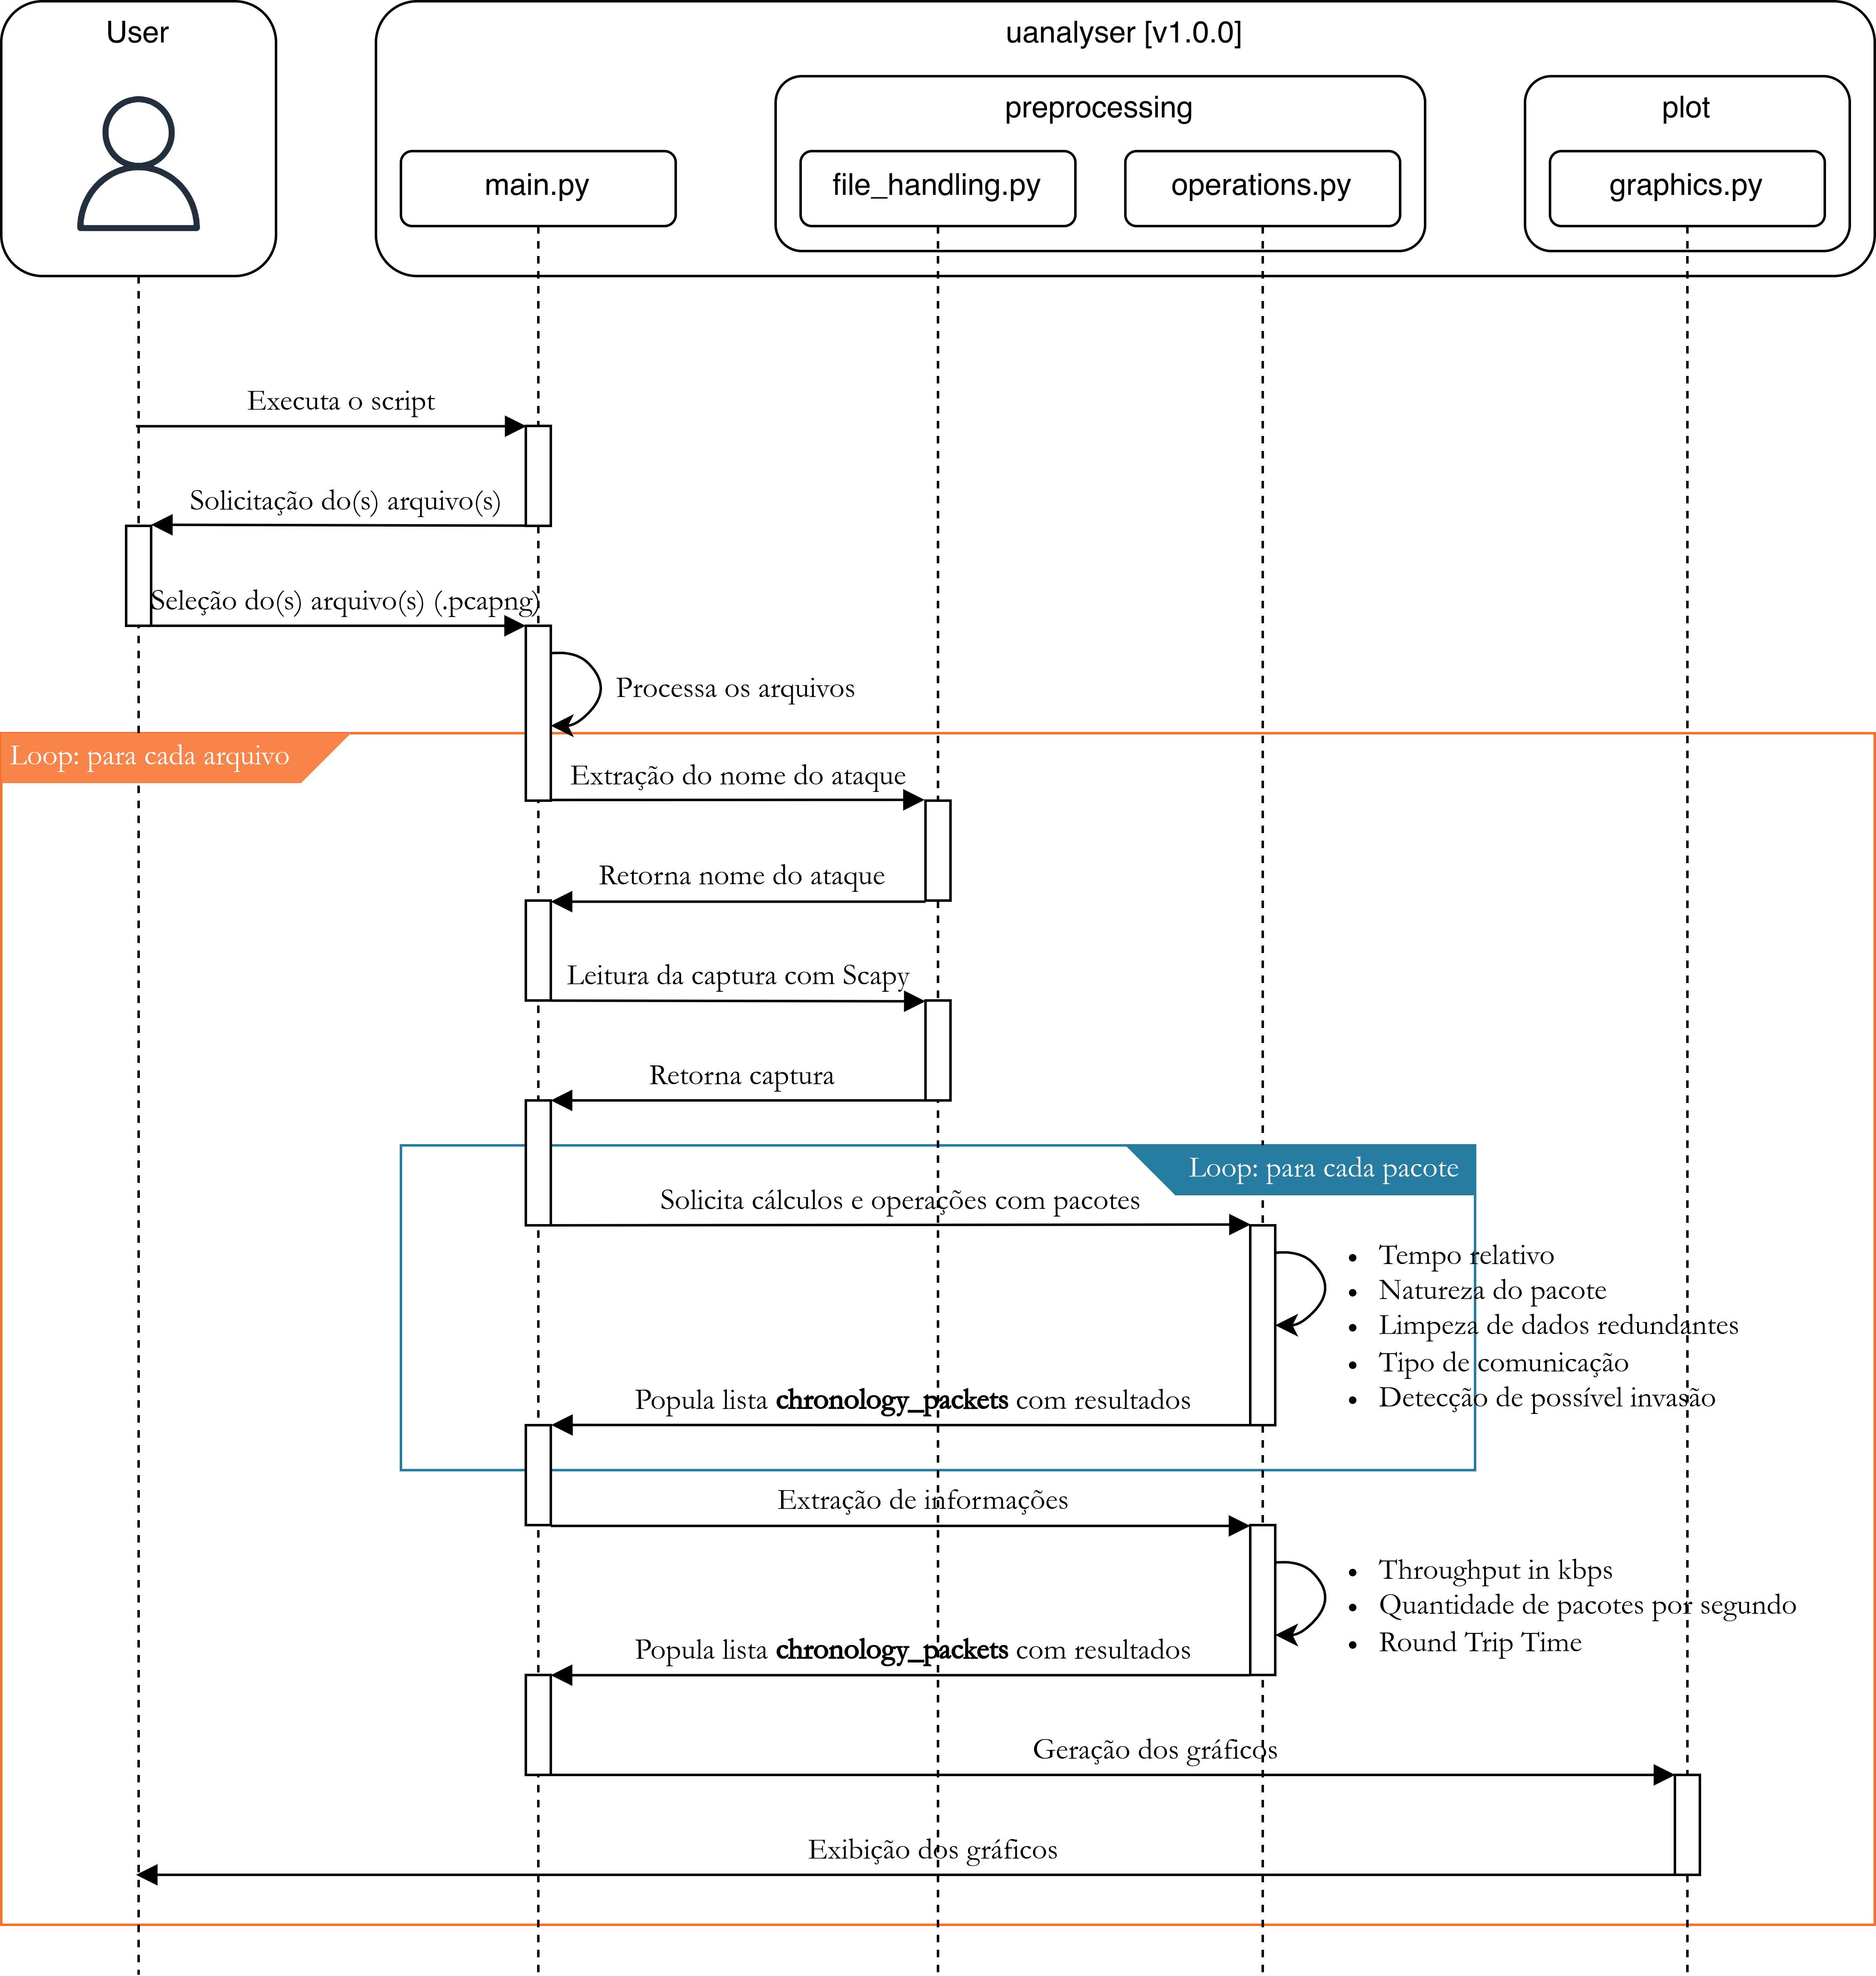
\includegraphics[width=0.972\textwidth]{USPSC-img/seqUanalyser.png}
            \end{center}
            \legend{Fonte: elaborada pelo autor.}
        \end{figure}

        No contexto do protocolo OPC UA, as mensagens trocadas entre cliente e servidor podem incluir diferentes estruturas de dados, como mensagens de sessão, mensagens de serviço e dados de publicação/subscrição. Cada tipo de mensagem possui seu próprio formato e estrutura, conforme definido pelo padrão OPC UA. A análise dessas mensagens é crucial para a identificação de comportamentos anômalos e potenciais vulnerabilidades.

        A análise dos pacotes capturados, associada à visualização dos gráficos gerados pelo \textbf{uanalyser}, permite uma compreensão aprofundada dos efeitos dos ataques em redes OPC UA. Essa abordagem sistemática e visual facilita a detecção de vulnerabilidades específicas do protocolo e contribui para o desenvolvimento de contramedidas eficazes, visando aprimorar a segurança e a resiliência das redes industriais.

        O software desenvolvido para este trabalho está disponível no GitHub\footnote{Disponível em: \url{https://github.com/JonathanTSilva/opcua-analyser}. Acesso em: 04 jul. 2024} e aberto a contribuições. Interessados em colaborar devem seguir as diretrizes estabelecidas no arquivo \texttt{contributing.md} e aderir ao código de conduta do projeto.


    \subsection{Análise dos Ataques e Vulnerabilidades}

        A análise de ataques e vulnerabilidades em redes industriais OPC UA é um processo sistemático e detalhado que tem como objetivo identificar, avaliar e mitigar possíveis fragilidades no protocolo e na implementação dessas redes. Essa etapa é essencial para garantir a segurança e a continuidade operacional dos IACS, sendo baseada na avaliação dos resultados obtidos a partir de testes e simulações de ataques cibernéticos conduzidos nas etapas anteriores. Cada tipo de ataque explora vulnerabilidades específicas, tanto no protocolo quanto na infraestrutura de rede.

        Ao investigar as vulnerabilidades na comunicação de redes industriais OPC UA, busca-se avaliar a qualidade da comunicação durante e após a ocorrência de um ataque. Em outras palavras, verifica-se se o equipamento mantém sua funcionalidade nesses períodos, além de analisar eventuais falhas, como ausência de resposta ou respostas anômalas por parte do sistema alvo.
        
        Dado que a análise de soluções existentes faz parte da abordagem deste estudo, é necessário estabelecer um referencial para avaliar as vulnerabilidades e o comportamento da rede durante os ataques. Com isso em mente, foram definidas as seguintes classes de vulnerabilidades para este projeto:
        
        \begin{itemize}
            \item \textbf{Classe 1}: falhas que interrompem a comunicação OPC UA entre os agentes, comprometendo a disponibilidade;
            \item \textbf{Classe 2}: interrupção de serviços ou comportamento inesperado que não afeta diretamente a comunicação, mas compromete a integridade;
            \item \textbf{Classe 3}: vulnerabilidades que não interrompem a comunicação, porém afetam a confiabilidade do sistema.
        \end{itemize}
        
        A partir da análise dos gráficos gerados e do comportamento da rede e dos dispositivos durante e após os ataques, torna-se possível identificar e classificar as vulnerabilidades conforme as categorias mencionadas. Além disso, avalia-se a eficácia das diferentes políticas de segurança do OPC UA (``None'', ``Sign'', ``Sign \& Encrypt''). A interpretação dos resultados obtidos é fundamental para detectar falhas potenciais e propor medidas corretivas e preventivas, visando a mitigação dos riscos de segurança em redes OPC UA.
        
        Essa abordagem metodológica, que inclui a análise de gráficos de \textit{throughput}, desempenho de RAM e CPU, quantidade de pacotes OPC UA por segundo e RTT normalizado, possibilita uma compreensão aprofundada do impacto dos ataques sobre as redes industriais OPC UA. Dessa forma, torna-se viável o desenvolvimento de estratégias de mitigação eficazes, garantindo maior robustez e resiliência contra ameaças cibernéticas.
    
    
    \subsection{Relatório de Vulnerabilidade}

        A construção de um relatório de vulnerabilidade é uma etapa fundamental no processo de avaliação da segurança cibernética, especialmente no contexto de redes industriais OPC UA. Esse relatório permite documentar e comunicar as vulnerabilidades identificadas, fornecer uma análise detalhada dos riscos e propor contramedidas adequadas. Além de viabilizar a compreensão das falhas de segurança, ele orienta a adoção de ações corretivas eficazes, contribuindo para o aprimoramento da postura de segurança da organização.

        A elaboração desse relatório deve seguir padrões internacionais de segurança cibernética e estar alinhada às melhores práticas do setor. Um relatório bem estruturado deve apresentar informações de forma clara e objetiva, contemplando diferentes níveis de detalhamento para atender a distintos públicos, desde executivos até equipes técnicas.
        
        O relatório de vulnerabilidade desempenha um papel essencial para diversos \textit{stakeholders} dentro da organização. Para os executivos, ele fornece uma visão geral da postura de segurança da empresa, auxiliando na justificativa de investimentos na área. Para a equipe de TI, apresenta detalhes técnicos sobre as vulnerabilidades descobertas e orientações para mitigá-las. Além disso, esse documento pode ser utilizado para fins de conformidade regulatória, sendo compartilhado com auditores e órgãos reguladores para demonstrar os esforços da organização na proteção de seus sistemas.
        
        Para garantir a eficácia do relatório de vulnerabilidade, ele deve incluir as seguintes seções principais:
        
        \begin{itemize}
            \item \underline{Sumário Executivo}: Visão geral de alto nível da avaliação, destinada a executivos não técnicos. Essa seção destaca as principais questões de segurança que podem impactar a organização, fornecendo subsídios para decisões estratégicas e ações corretivas prioritárias;
            \item \underline{Visão Geral}: Seção voltada para um público técnico, que apresenta um resumo da avaliação. Deve incluir informações sobre os sistemas analisados, as ferramentas utilizadas e uma classificação preliminar das vulnerabilidades identificadas, considerando sua severidade e impacto;
            \item \underline{Detalhes da Avaliação}: Apresenta uma descrição técnica detalhada do processo de avaliação de vulnerabilidades. Deve documentar as metodologias empregadas, as etapas realizadas e os resultados obtidos, permitindo a replicação dos testes e a validação das descobertas;
            \item \underline{Resultados}: Seção dedicada à apresentação detalhada das vulnerabilidades identificadas. Cada vulnerabilidade deve ser classificada por severidade, destacando os problemas mais críticos. Devem ser fornecidas informações sobre os sistemas afetados, a categorização da vulnerabilidade, seu impacto potencial e referências adicionais, como identificadores CVE;
            \item \underline{Mitigações Recomendadas}: O objetivo da avaliação de vulnerabilidades é auxiliar a organização na melhoria de sua postura de segurança. Assim, esta seção deve apresentar recomendações para mitigação dos riscos identificados. As sugestões podem envolver a aplicação de atualizações de segurança, o fortalecimento de credenciais ou a reconfiguração de parâmetros críticos do sistema.
        \end{itemize}
    
        Uma vez elaborado, o relatório de vulnerabilidade deve ser incorporado às bases de conhecimento da organização, garantindo que todas as vulnerabilidades identificadas sejam tratadas de forma adequada. Além disso, o documento deve ser revisado periodicamente e atualizado sempre que novas vulnerabilidades forem descobertas ou medidas corretivas forem implementadas. Para assegurar a consistência e a confiabilidade das informações, é fundamental que o relatório esteja alinhado com padrões globais de cibersegurança, como o CVE (do inglês \textit{Common Vulnerabilities and Exposures}) e as normas de segurança IEC 62443.

        A adoção de frameworks reconhecidos internacionalmente, como o CVE e a IEC 62443, fornece uma base sólida para a identificação e classificação de vulnerabilidades. Esses padrões estabelecem diretrizes claras para a avaliação e mitigação de riscos, promovendo práticas de segurança consistentes e eficazes. Além disso, diversos modelos são amplamente utilizados na elaboração de relatórios de vulnerabilidade, como os da CISA (do inglês \textit{Cybersecurity and Infrastructure Security Agency}) e do NIST (do inglês \textit{National Institute of Standards and Technology}), os quais podem ser adaptados para atender às necessidades específicas de cada organização. Caso seja identificada uma vulnerabilidade desconhecida no protocolo OPC UA, será utilizado um modelo de relatório personalizado, disponível no \autoref{ap:relatorio}, para documentar e comunicar a descoberta de maneira estruturada e detalhada.

    \subsection{Contramedidas de Segurança}

        A implementação eficaz de contramedidas de segurança é uma das principais estratégias para mitigar riscos cibernéticos e assegurar a disponibilidade, integridade e confidencialidade dos Sistemas de Automação e Controle Industrial. A proteção das redes industriais baseadas no protocolo OPC UA deve adotar uma abordagem holística, abrangendo não apenas a proteção dos ativos de informação, mas também a prevenção de ameaças e a detecção e resposta a incidentes.
        
        A definição das contramedidas apropriadas depende do cenário de ataque e das vulnerabilidades identificadas. Entretanto, algumas práticas amplamente reconhecidas podem ser implementadas para fortalecer a segurança das redes OPC UA. Dentre as principais contramedidas recomendadas, destacam-se:
        
        \begin{itemize}
            \item \underline{Criptografia e modos de segurança:} em conformidade com as políticas de segurança ``Sign'' e ``Sign \& Encrypt'', a aplicação de criptografia e assinatura digital na comunicação OPC UA representa uma das medidas mais relevantes para aprimorar a segurança. Essa abordagem inclui a utilização de certificados digitais robustos e algoritmos criptográficos atualizados para garantir a confidencialidade e autenticidade dos dados transmitidos. Além disso, é essencial a renovação periódica de certificados e a adoção de mecanismos de revogação para mitigar o impacto de comprometimentos de chaves criptográficas;
            \item \underline{Autenticação reforçada:} a implementação de mecanismos de autenticação forte para acesso ao servidor OPC UA é fundamental para restringir acessos não autorizados. Métodos como autenticação multifator (MFA, do inglês \textit{Multi-Factor Authentication}) e a autenticação baseada em certificados digitais elevam o nível de segurança ao validar a identidade de usuários e dispositivos. A autenticação baseada em credenciais padrão (usuário e senha) deve ser evitada ou, quando necessária, associada a políticas rigorosas de complexidade e expiração de senhas;
            \item \underline{Segmentação e proteção da rede:} a criação de zonas de segurança na rede industrial limita a propagação de ataques, seguindo o modelo de defesa em profundidade (do inglês \textit{Defense in Depth}). Cada zona deve ser protegida por \textit{firewalls} e dispositivos de segurança que monitoram e controlam o tráfego de dados. Além disso, a adoção do modelo \textit{Zero Trust}, fundamentado no princípio de ``nunca confiar, sempre verificar'', reforça a necessidade de autenticação e autorização rigorosas para todas as tentativas de acesso, independentemente da origem. A implementação de redes definidas por software (SDN, do inglês \textit{Software-Defined Networking}) também pode auxiliar na criação de regras dinâmicas de segmentação, reduzindo a superfície de ataque;
            \item \underline{Controle de Acesso Baseado em Função (RBAC, do inglês \textit{Role-Based Access Control})} a implementação de RBAC permite restringir o acesso a recursos críticos exclusivamente a usuários e dispositivos autorizados, reduzindo significativamente o risco de acessos indevidos. Essa abordagem garante que cada entidade tenha permissões compatíveis com suas responsabilidades operacionais. O RBAC pode ser complementado com o ABAC (do inglês \textit{Attribute-Based Access Control}), permitindo regras de acesso baseadas em atributos contextuais, como horário, localização ou dispositivo utilizado;
            \item \underline{Monitoramento contínuo e resposta a incidentes:} a detecção precoce de atividades anômalas é essencial para a segurança cibernética das redes OPC UA. A implementação de sistemas de detecção de intrusão (IDS, do inglês \textit{Intrusion Detection Systems}) e de gerenciamento de eventos e informações de segurança (SIEM, do inglês \textit{Security Information and Event Management}) possibilita a identificação e análise de padrões de comportamento suspeitos. Além disso, um plano estruturado de resposta a incidentes, baseado em boas práticas da norma IEC 62443, define procedimentos claros para contenção, erradicação e recuperação de ataques cibernéticos. A utilização de inteligência artificial e aprendizado de máquina para análise de tráfego e predição de ameaças pode aprimorar a capacidade de detecção e mitigação de ataques sofisticados;
            \item \underline{Aplicação de atualizações e correções de segurança:} a manutenção da segurança dos sistemas requer a atualização regular de servidores OPC UA, dispositivos de rede e sistemas operacionais com os últimos \textit{patches} de segurança disponibilizados pelos fornecedores. Essa prática reduz a exposição a vulnerabilidades conhecidas e previne possíveis explorações. O uso de ferramentas de gerenciamento de vulnerabilidades permite a identificação e priorização de correções críticas, garantindo a aplicação eficiente das atualizações;
            \item \underline{\textit{Hardening} de sistemas:} a aplicação de técnicas de \textit{hardening} visa minimizar a superfície de ataque dos servidores e dispositivos de rede, tornando-os menos suscetíveis a explorações. Isso inclui a desativação de serviços desnecessários, a configuração segura de sistemas operacionais e aplicações, e a implementação de políticas de segurança rigorosas. Além disso, a utilização de ambientes de execução isolados, como \textit{containers}, pode reduzir os impactos de possíveis comprometimentos;
            \item \underline{Educação e treinamento em segurança:} a segurança cibernética de redes industriais não depende exclusivamente de soluções tecnológicas, mas também do fator humano. Programas contínuos de capacitação para operadores, engenheiros e administradores de sistemas são essenciais para disseminar boas práticas de segurança. Simulações de ataques e exercícios de resposta a incidentes podem aumentar a conscientização e preparar a equipe para lidar com ameaças reais;
            \item \underline{Gestão de segurança baseada em normas e conformidade regulatória:} a adesão a frameworks de segurança reconhecidos internacionalmente, como a norma IEC 62443, o NIST Cybersecurity Framework e as diretrizes da ISO/IEC 27001, fortalece a governança e a resiliência das redes OPC UA. Auditorias periódicas e avaliações de conformidade garantem que as práticas de segurança estejam alinhadas com os requisitos regulatórios e as melhores práticas do setor.
        \end{itemize}
        
        A definição e implementação dessas contramedidas exigem um processo contínuo de avaliação de riscos, monitoramento de ameaças emergentes e adequação às melhores práticas de cibersegurança. A combinação de uma análise detalhada de vulnerabilidades, a adoção de frameworks de segurança reconhecidos e a implementação de medidas de mitigação bem estruturadas contribui para a proteção robusta das redes industriais OPC UA. Dessa forma, este trabalho busca fortalecer a resiliência dos sistemas críticos, mitigando ameaças cibernéticas e garantindo a segurança operacional em um ambiente industrial cada vez mais conectado e dinâmico.
        
        Além das estratégias descritas, o avanço das ameaças cibernéticas exige uma abordagem proativa, com a utilização de ferramentas avançadas de detecção e resposta, bem como a integração de inteligência artificial para prever e mitigar ataques antes que causem impactos significativos. O cenário de segurança em redes OPC UA está em constante evolução, e a implementação de medidas adaptáveis e eficazes será essencial para enfrentar desafios futuros. Dessa forma, este estudo reforça a necessidade de uma governança de segurança cibernética robusta, garantindo a confiabilidade e a disponibilidade dos sistemas industriais em um contexto de ameaças cada vez mais sofisticadas.
    


    